% setwd(path <- "c:/seiro/docs/external/seishin/lec_slides/2024/"); system("recycle c:/seiro/docs/external/seishin/lec_slides/2024/cache/1"); library(knitr); knit("1.rnw", "1.tex"); system("platex 1"); system("pbibtex 1"); system("dvipdfmx 1")

\input{c:/seiro/settings/Rsetting/knitrPreamble/knitr_beamer_preamble169.rnw}
%\input{c:/seiro/settings/Rsetting/knitrPreamble/knitr_beamer_preamble169_ho.rnw}

\usepackage[xcolor, framemethod=TikZ]{mdframed}
\mdfsetup{%
  middlelinecolor=blue!30,
  middlelinewidth=1.5pt,
  backgroundcolor=blue!05,
  roundcorner=10pt
  }
\definecolor{bondiblue}{rgb}{0.0, 0.58, 0.71}
\definecolor{bondibluelight}{rgb}{0.0, 0.3, 0.41}
\definecolor{aqua}{rgb}{0.0, 1.0, 1.0}
\definecolor{bittersweet}{rgb}{1.0, 0.44, 0.37}
%\setbeamercolor{background canvas}{bg=bondibluelight}
\setbeamercolor{background canvas}{bg=darkdarkblue}
\setbeamercolor{normal text}{fg=white}
\setbeamercolor{item}{fg=aqua}
\mode<handout>{\setbeamercolor{item}{fg=blue!70!black}}
\mode<handout>{\setbeamercolor{background canvas}{bg=white}}
\mode<handout>{\setbeamercolor{normal text}{fg=black}}
\hypersetup{
%linkcolor = lightblue, urlcolor = lightblue
linkcolor = blue!50, urlcolor = green!80
, citecolor = blue!50
}
\setbeamercovered{invisible}
\newcommand{\DescPause}{\hspace{-.25em}\phantom{\thebeamerpauses}\pause}

\usepackage{tikz-qtree, tikz-qtree-compat}
\usepgfplotslibrary{fillbetween}
\pgfplotsset{compat=1.10}
\colorlet{DarkGreen}{green!50!black}


\begin{document}
\setlength{\baselineskip}{12pt}







\title[1]{\large はじめに}
\author[Ito]{伊藤成朗}
\institute[SHU, IDE]{聖心女子大学\\ アジア経済研究所}
\date[2022秋学期]{2022年秋学期\\\vspace{1ex} 国際交流学科}
\logo{SHU, IDE}


\frame{\titlepage}
\setcounter{page}{1}

%\setbeamercovered{transparent = 40}
%\setbeamercolor{normal text}{fg=turquoiseblue2, bg=}
%\setbeamercolor{alerted text}{fg=black, bg=}
%\usebeamercolor{normal text}


\begin{frame}{}
本講義の目的: 以下を実施すること。Purposes of this course: To
\begin{itemize}[<+->]
\vspace{1.0ex}\setlength{\itemsep}{3.0ex}\setlength{\baselineskip}{12pt}
\item	低所得国で貧困を生むメカニズムを知ること。Know the mechanism that generates poverty in low income countries.
\item	身の回りの社会経済課題についての論理的・経済学的思考方法に習熟すること。Be familiar with logical and economic thinking on socioeconomic issues around us.
\item	因果関係の推論方法を知ること。Know how to infer causal relationships.
\item	データ視覚化の方法を知ること。Know how to visualise data.
\item	開発ミクロ経済学の入門的知識を得ること。Get an accessible introduction to development microeconomics.
\item	研究の最先端を垣間見ること。Have a glimpse of research frontier.
\end{itemize}
\end{frame}


\begin{frame}{}
トピック: Topics: 
\begin{itemize}[<+->]
\vspace{1.0ex}\setlength{\itemsep}{1.0ex}\setlength{\baselineskip}{12pt}
\item	家計: 消費、家計内資源配分、労働供給、人的資本、早期児童発達、リスク、認知バイアスと変則行動など。
\item	Households: Consumption, intrahousehold resource allocation, labour supply, human capital, early childhood development, risks, cognitive biases and behavioral anomalies, etc.
\item	企業: 物的資本、信用制約、起業家能力と経営資本など。
\item	Firms: Physical capital, credit constraints, entrepreneurship and management capital.
\item	可能な限り多く扱う。
\item	Hope to cover as many as possible.
\end{itemize}
\end{frame}


\begin{frame}{ハウスキーピングhousekeeping}
成績: 下記のウェイトを使います。
\begin{description}
\vspace{1.0ex}\setlength{\itemsep}{1.0ex}\setlength{\baselineskip}{12pt}
\item[クラス内短試験] 10\%. $\rightarrow$ オンラインでは実施不可だったので、質問や発言によるクラスへの貢献度で代替
\item[宿題、レポート] 3-4 times, 50\% or more.
\item[クラス内参照可能期末試験In-class, open book (web), final exam] Up to 40\%. 
\item[希望者のみレポートOptional reports] 20\%.
\end{description}
希望者のみレポート以外で100になるようにする。希望者のみレポートは100に加算。
\begin{itemize}
\vspace{1.0ex}\setlength{\itemsep}{1.0ex}\setlength{\baselineskip}{12pt}
\item	レポートはグループ作業も歓迎します。その際には共同作業した学生の名前を明記し、文章は各自が書くようにして下さい。文章を参照記載なしに複製した場合には、点数は共有にします(=1名分の点数を複製した人数で割ります)。
\item	期限を過ぎた提出は成績に反映されません。
\end{itemize}
\end{frame}

\begin{frame}{ハウスキーピングhousekeeping}
その他: Other stuffs:
\begin{itemize}
\vspace{1.0ex}\setlength{\itemsep}{1.0ex}\setlength{\baselineskip}{12pt}
\item	オフィスはありませんので、質問等は講義の後にオンラインで直接、もしくは、その他の時間にメールでお願いします。 seiroi@gmail.com
\item	\textcolor{red}{クラス内の質問を推奨します。}
\item	講義言語: 日本語
%\item	\sout{I may or may not have to reschedule a class or two in January.}
\item	リアクション・ペーパーを講義終了日の20時までにGoogle Classroomにアップロード。時間の猶予がほしい場合には都度ご相談下さい。Hard copy?
%	\item	下記を書いて頂けると助かります。
	\begin{itemize}
	\vspace{1.0ex}\setlength{\itemsep}{1.0ex}\setlength{\baselineskip}{12pt}
	\item	感想
	\item	分かりづらかった点
	\item	こういう理解で良いかという確認
	\item	参考文献照会
	\item	その他疑問など
	\end{itemize}
\end{itemize}
\end{frame}

\begin{frame}[t]{今回のトピック}
開発経済学の動機\\~\\
経済学の動機\\~\\
開発経済学の今まで\\~\\
開発の概観\\~\\
貧困の罠\\~\\
ランダム化比較試験RCT
\end{frame}

\begin{frame}{}
\begin{description}
\setlength{\itemsep}{3.0ex}\setlength{\baselineskip}{12pt}
\item[開発経済学とは?] \DescPause 発展地域を分析する経済学の一分野。
\pause
\item[クラスで習う普通の経済学と違うものですか?]\DescPause 同じです。 
\pause
\item[では、なぜ開発経済学が必要なのですか?] \DescPause
必要かどうかには議論があります。特別な経済学は必要ないかもしれませんが、発展地域の課題の特性を分析する経済学は必要です。
\pause
\item[開発経済学と普通の経済学に違いがあるとすれば何ですか?] \DescPause
発展地域を扱うので、対象にする個人、家計、経済取引、保健や環境の課題、社会習慣やルールなどが違います。普通の経済学を使ってこれらを分析しますが、先進地域とは異なる視点や仮定の下で分析します。経済学は人々の意思決定を説明しようとしていることを思い出して下さい。そうした道具を異なる社会経済条件下の人々、企業、組織、政府などに適用します。これが開発経済学の中身です。
\end{description}
\end{frame}
\begin{frame}{}
\begin{description}
\setlength{\itemsep}{1.0ex}\setlength{\baselineskip}{12pt}
\item[What is development economics?]\pause 	It is a branch of economics that studies the developing areas.
\pause
\item[Is it different from regular, economics that we learn in a class?]\pause 	No. 
\pause
\item[Then, why do we need development economics?]\pause 	There is a debate if we need one. We may not need a special economics, but we definitely need economics to understand the nature of problems in developing areas. 
\pause
\item[What is special about development economics?]\pause  Because it deals with developing areas, we study a very different set of individuals, households, economic transations, health issues, environmental issues, social customs, rules, etc. While we still use economics as a tool to analyse issues, we need a different set of perspectives and assumptions than when we analyse issues of developed areas. Remember, economics tries to explain about people's decision making. We apply it to the people, firms, groups, organizations, governments of different countries under different socioeconomic conditions.  That is the content of development economics.
\end{description}
\end{frame}

\begin{frame}{}
今後学ぶ内容がぼんやりと分かったと思います。Now, you have a very vague picture of what you will learn.\\~\\
\pause
では、開発経済学をどのように役立てるか問うて下さい。Then, please ask yourself what you make out of dev econ.\\~\\
\pause
違う言い方をすれば、あなたが開発経済学を学ぶ根源的な動機です。Or, your intrinsic motivation of studying dev econ.\\~\\
\pause
以下では動機を1つ挙げることができます。I can give you one good motivation. \\~\\
\pause
\textcolor{red}{われわれの共感能力が不完全であるため}です。Our imperfect empathy.
\end{frame}

\begin{frame}[label=PeterSinger]{}
\begin{columns}[T]
\column{.6\textwidth}
Peter Singer、倫理学者、哲学者 \url{https://petersinger.info/projects} \\~\\
\pause
\textit{溺れる子どもChild in the pond}問題:\\~\\
\hfill\hyperlink{PeterSingerEnglish}{\beamergotobutton{ChildInThePond}}
\column{.4\textwidth}
\hfil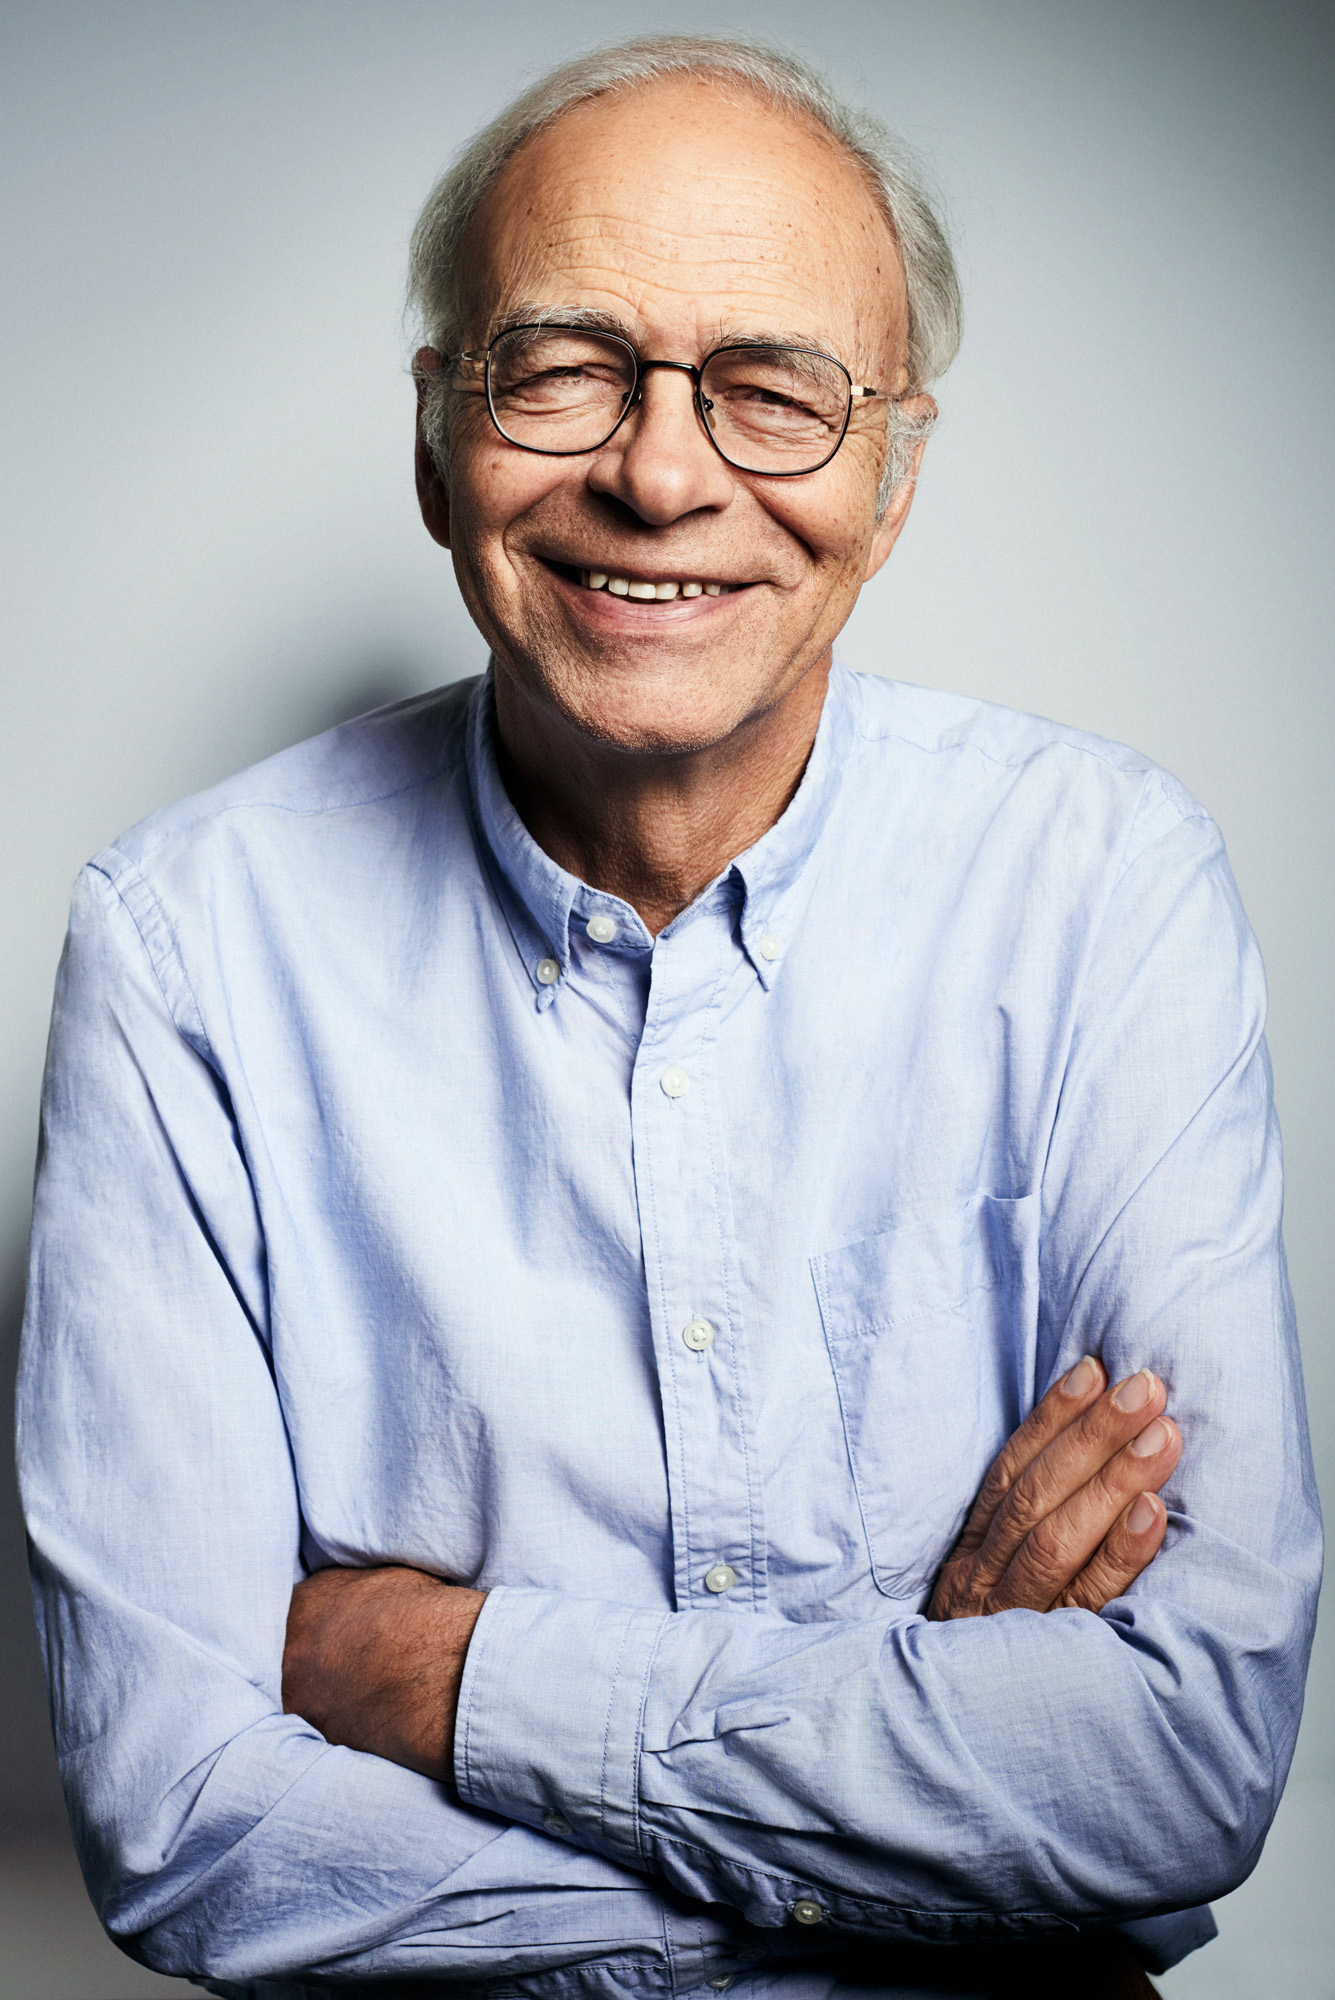
\includegraphics[height = 2cm]{c:/seiro/docs/external/seishin/lec_slides/2024/1/PeterSinger.jpg}\\
\hfil{\scriptsize Photo by Alletta Vaandering}
\end{columns}
\pause
ほぼ全員が「はい」\\~\\
\pause
シンガーの問い\\~\\
\pause
シンガー: 先進国に住むわれわれは所得の一定割合を貧しい国の住民に与える道徳的義務がある\\~\\
\pause
\begin{dinglist}{43}
\vspace{1.0ex}\setlength{\itemsep}{1.0ex}\setlength{\baselineskip}{12pt}
\item	われわれは共感する人間でありたい、貧しい国の貧困について考えたい、と思っているはずですが、かなり不完全にしかできません。(だから、強制的に考えるように仕向けなければならない、のかもしれない。)なぜ貧しいか、何で困っているか、を理解することが、共感を行動に変える第一歩になると思います。
\end{dinglist}
\end{frame}

\begin{frame}[t, label=DenisMukwege]{}
\begin{columns}[T]
\column{.6\textwidth}
Denis Mukwege、婦人科医、ノーベル平和賞受賞者 {\scriptsize\url{https://www.mukwegefoundation.org/dr-denis-mukwege/}} \\~\\
DRCでの(戦争)暴力被害者女性の治療と啓発活動\\
\hyperlink{https://www.nhk.jp/p/ts/X83KJR6973/episode/te/VW23V46YQ4/}{NHKこころの時代「沈黙は共犯 闘う医師」}
\column{.4\textwidth}
\hfil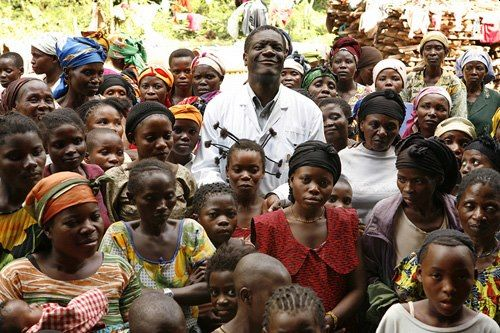
\includegraphics[height = 3cm]{c:/seiro/docs/external/seishin/lec_slides/2024/1/DenisMukwege.jpg}\\
\hfil{\scriptsize Photo by MONUSCO CC BY-SA 2.0} \includegraphics[height = .45cm]{c:/seiro/docs/external/seishin/lec_slides/2024/1/cc-by-sa_nobackground.jpg}\\
\end{columns}
\pause
\vspace{2ex}
戦争・災害が起こると暴力が始まる\pause$\leftarrow$平和時から暴力の根がある\\~\\
\pause
反無関心: (性)暴力、戦争での殺戮は被害者を物として捉えることで可能になる\\~\\
\pause
非紛争地でも平時から他者への尊敬と差別を許さない行動: 暴力を減らせる\\~\\
\pause
\begin{dinglist}{43}
\vspace{1.0ex}\setlength{\itemsep}{1.0ex}\setlength{\baselineskip}{12pt}
\item	暴力はどこの社会でも発生するので、行動は自分の周囲でいい
\end{dinglist}
\end{frame}

\begin{frame}[t, label=Rawls]{}
\begin{columns}[T]
\column{.5\paperwidth}
John Rawls、政治哲学者 {\scriptsize\url{}} \\~\\
\pause
「正義論」A theory of justiceで許容できる不平等を問うた
\column{.45\paperwidth}
\hfil\mpage{.4\paperwidth}{\mpagethree{.1\paperwidth}{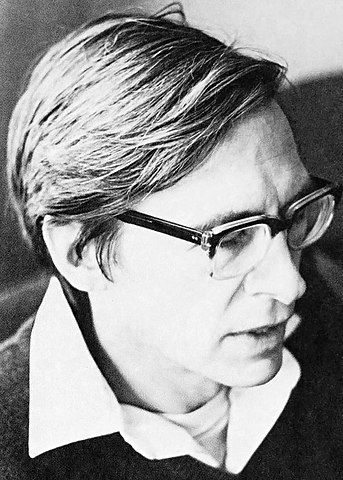
\includegraphics[width = .1\paperwidth]{c:/seiro/docs/external/seishin/lec_slides/2024/1/JohnRawls.jpg}}{c}\mpagethree{.2\paperwidth}{\hfil{\scriptsize Photo by Alec Rawls}\\\hfill
\includegraphics[height = .5cm]{c:/seiro/docs/external/seishin/lec_slides/2024/1/PublicDomain.jpg}}{c}} \\
\end{columns}

\vspace{2ex}
\pause
\textit{Original positionによる思考実験:} People deliberately select what kind of society they would choose to live in if they did not know which social position they would personally occupy. \\~\\
\pause
\textit{Veil of ignorance:} OP思考実験では、自分が社会のどの地位を占めるか分からないと想定。
\begin{dinglist}{43}
\vspace{1.0ex}\setlength{\itemsep}{1.0ex}\setlength{\baselineskip}{12pt}
\pause
\item	性別、宗教、人種、年齢、知力、財力などについて分からない
\end{dinglist}
\vspace{2ex}
%\pause
%この想定下で各人が許容できる分配の不平等を問うた\\~\\
\pause
特定のグループを差別する分配は誰も提案しないし、最悪の状態にある人たちを救おうとする\\~\\
\pause
\begin{dinglist}{43}
\vspace{1.0ex}\setlength{\itemsep}{1.0ex}\setlength{\baselineskip}{12pt}
\item	自分が恵まれない条件化にあるかもと思えば助けたくなる
\end{dinglist}
\end{frame}

\begin{frame}[t, label=SingerMukwegeRawls]{}
シンガー: 地球の裏側まで共感せよ\\~\\
ムクウェゲ: 共感は自らの周囲からでいい、共感するために平時から他者の尊敬と差別撤廃\\~\\
ロウルズ: 共感すべき理由=無知のヴェイル\\~\\
\pause
開発経済学はどのような条件の下に置かれているかを理論モデルのなかに位置づけ、(機会平等を期するために)どのような介入が必要か考える\\~\\
\pause
共感能力が乏しくても、論理的に整理することて、問題を理解して解決策を提示できる
\end{frame}

\begin{frame}[t, label=AnotherMotivation]{}
開発経済学を学ぶ動機をもう1つ挙げられます。\\~\\
\pause
\textcolor{red}{世界を豊かにするため}です。\\~\\
\pause
インドには10億人以上の人がいます。
\pause
その20\%前後が文盲です。
\pause
2億人が追加的に識字人口に加わると世界はどう変わるでしょうか。\\~\\
\pause
識字人口1億人に1人が素晴らしい発見をすると仮定すると、素晴らしい発見が2個増えます。\\~\\
\pause
インドは若年人口が半分以上を占め、5億人の20\%である1億人が大卒になるとし、その1000万人に1人が素晴らしい発見をすれば、発見は10個増えます。\\~\\
\pause
新たな12個の素晴らしい発見によって、世界は豊かになり、あなたの生活も豊かになります。
\begin{dinglist}{43}
\vspace{1.0ex}\setlength{\itemsep}{1.0ex}\setlength{\baselineskip}{12pt}
\pause
\item	知識(発見)は廃れず誰でも使えます。公共財。
\pause
\item	知識生産に関わる人が多いほど所得の成長率は高まります\citep{Kremer1993}。知識生産人口が減少すると成長しなくなります\citep{Jones2022}。
\end{dinglist}
\end{frame}

\begin{frame}{}
I want you to rise above the cycle of punishments and rewards.\\~\\
\pause
This [my teaching] is information, and you can do what you want with this information.\\~\\
\pause
If you want to learn something, I cannot stop you.\\
\pause
If you do not want to learn it, I cannot teach you.\\~\\

\pause
\hfill Wynton Marsalis, a jazz trumpeter,\\
\hfill a teacher/director of Juilliard Jazz Studies program\\
\hfill\href{http://freakonomics.com/archive/}{\textit{Freakonomics Radio}}, Episode 355, 01:16:30.
\end{frame}


\begin{frame}{}
\hfil\href{https://wyntonmarsalis.org/images/press/TwoMenWithTheBlues_cover_back.jpg}{Wynton}
\end{frame}


\begin{frame}{}
開発経済学は普通の経済学と同じ分析道具を使います。\\~\\

よって、先進地域を学ぶことで発展途上地域を分析する技術を磨くことができます。\\~\\

役に立つと思えるときには、日本をはじめとする先進地域の課題も取り上げます。\\
%I will use mostly Japanese for the topics on Japan.
\end{frame}

\begin{frame}{}
経済学を使って課題を理解することの利点は何でしょうか。\\~\\
\pause
経済学はどのように人々が(よって社会が)変化に対して反応するか明らかにできます。ときには、意図せざる結果になることもあります。\\~\\
\pause
変化に伴う資源配分の効率性(無駄が増えるか減るか)も議論します。
\end{frame}

\begin{frame}[label=ChinaClamSchool]{}
例1: 中国の塾授業料上限規制\\
\begin{columns}[T]
\column{.6\textwidth}
  \centering
\begin{tikzpicture}[inner sep=0pt, remember picture]
\node at (0, 0) {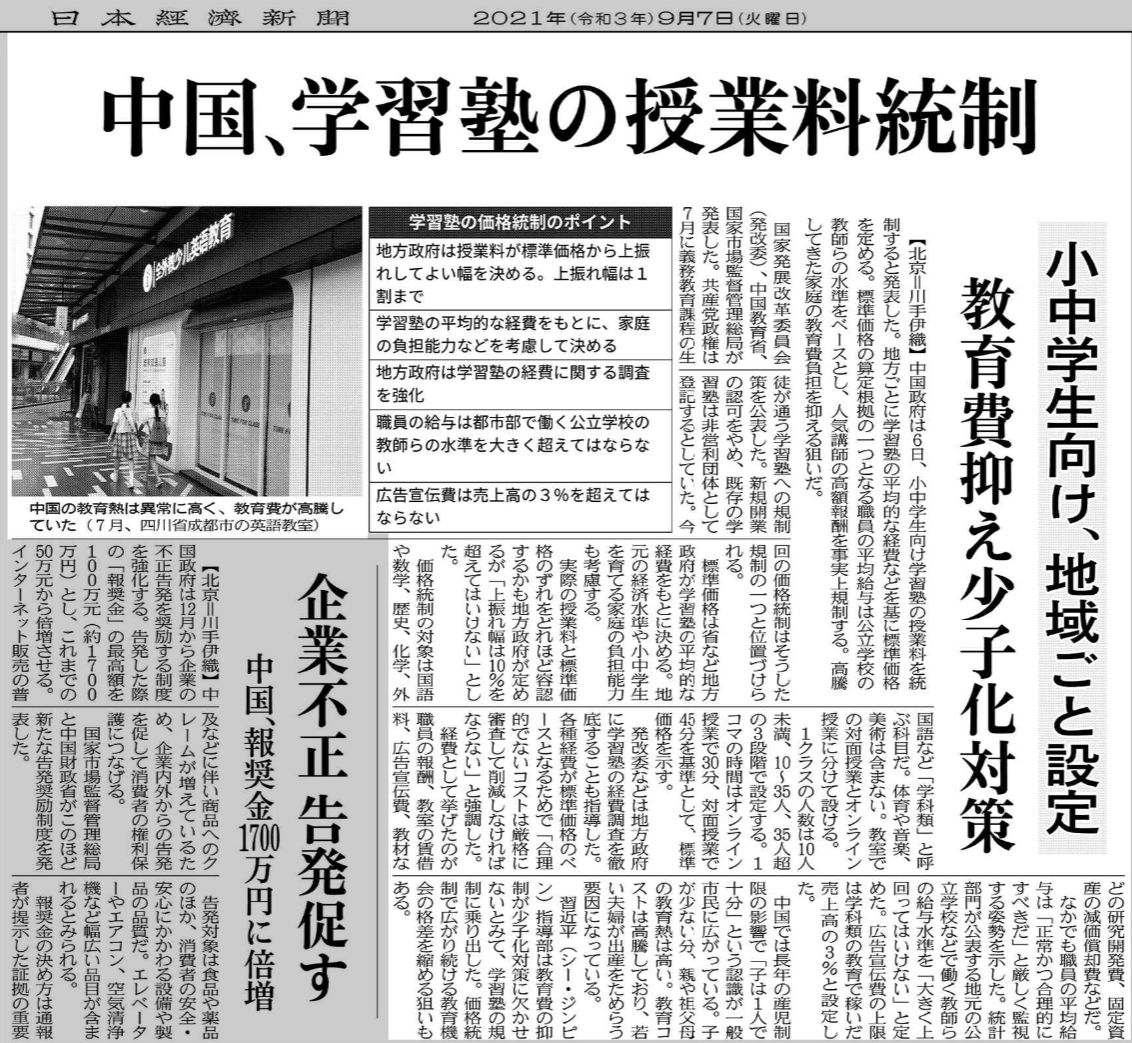
\includegraphics[width = .9\textwidth]{c:/seiro/docs/external/seishin/lec_slides/2024/1/ChinaClamSchoolFeeControl_Nikkei20201Sep07.jpg}};
\onslide<2->{\node (a) [draw, rectangle, thick, rounded corners, minimum height = 1.25cm, minimum width = .5cm, red] at (1.05cm, .5cm){};
}
\end{tikzpicture}

\column{.4\textwidth}
%   \hspace{-10em}\begin{description}
%   \vspace{1.0ex}\setlength{\itemsep}{1.0ex}\setlength{\baselineskip}{12pt}  
%   \setlength{\labelwidth}{-3em}
%   \setlength{\itemindent}{-4em}
%   \item[目的]  家計の教育費を抑え、養育費用を下げて出産増加を狙う。
%   \item[手段]  (塾の収入)授業料上限を設定。(塾の支払)塾講師賃金や広告宣伝費に上限を設定。
%   \end{description}
  \begin{itemize}
  \vspace{1.0ex}\setlength{\itemsep}{1.0ex}\setlength{\baselineskip}{12pt}
  \item[目的]  家計の教育費を抑え、養育費用を下げて出産増加を狙う。
  \item[手段]  (塾の収入)授業料上限を設定。(塾の支払)塾講師賃金や広告宣伝費に上限を設定。
  \item	授業料を下げると、塾は? 家計は?
  \item	賃金や広告宣伝費を下げると塾は?\\~\\
  \end{itemize}
  中国共産党は塾への統制で少子化を防ぐことができるでしょうか。\\~\\
  \begin{tikzpicture}[inner sep=0pt, remember picture]
  \node (b) at (0, 0) {\footnotesize * 非営利団体に登記、とはすごい...};
  \end{tikzpicture}
\end{columns}

\onslide<2->{
\begin{tikzpicture}[remember picture, overlay]
\draw[red, very thick, ->] (b.west) to [out=180, in=-90] (a.south);
\end{tikzpicture}
}
\end{frame}

\begin{frame}[label=ChinaDemandSupply]{}
\begin{columns}[T]
\column{.7\textwidth}
\hfil\begin{tikzpicture}[ 
axis/.style={very thick, ->, >=stealth'},
dashed line/.style={dashed, thin},
every node/.style={color=white!70!blue},
background rectangle/.style = {fill = gray90},
]
\begin{axis}[
  scale = 1.5,
  axis equal image, % forces a square plot
  clip = false, % allows plotting outside axis bounds
  axis x line=center, axis y line=center,
  xlabel = {量$x$}, ylabel = {価格$p$},
  xtick={100}, ytick={100}, % effectively drops axis ticks
  xlabel style={below right}, ylabel style={above left},
  xmin=0, xmax=11,
  ymin=0, ymax=10]
\path[name path=xaxis] (0, 0) -- (10, 0);
\path[name path=yaxis] (0, 0) -- (0, 10);
\coordinate (origin) at (0, 0);
\coordinate (i11) at (axis cs: .5, 9);
\coordinate (i12) at (axis cs: 1.0, 6);
\coordinate (i13) at (axis cs: 2.0, 4);
\coordinate (i14) at (axis cs: 4, 3);
\coordinate (i15) at (axis cs: 8, 2);
\coordinate (e1) at (axis cs: 1.75, 4.4);
\coordinate (e2) at (axis cs: 3.25, 2.25);
\coordinate (a) at (axis cs: 0, 7);
\coordinate (c) at (axis cs: 6, 1);
\coordinate (b) at (axis cs: 0, 1);
\coordinate (d) at (axis cs: 7, 6);
\node[left] (dum1) at (axis cs: 0, 2) {\phantom{$p^{*}$}};
\node[below] (dum2)  at (axis cs: 2, 0) {\phantom{$x^{*}$}};
\node at (axis cs: 7.5, 10) {\phantom{\mpage{6cm}{需要曲線$D$は右下がり\\ $\Rightarrow$ 消費者は価格が低いと買いたい量も増えるため}}};
\only<2->{
  \draw[name path=Dline1, color = green, line width = 1.5pt] 
  plot coordinates {(a) (c)} node[right]{$D$};
  \node at (axis cs: 7.5, 10) {\mpage{6cm}{需要曲線$D$は右下がり\\ $\Rightarrow$ 消費者は価格が低いと買いたい量も増えるため}};}
\only<3->{
  \node at (axis cs: 7.5, 7.5) {\mpage{6cm}{供給要曲線$S$は右上がり\\ $\Rightarrow$ 生産者は価格が高いと売りたい量も増えるため}};
  \draw[name path=Sline1, color = blue, line width = 1.5pt] 
    plot coordinates {(b) (d)} node[right]{$S$};}
\only<4->{
  \path [name intersections={of=Dline1 and Sline1, by={e}}];
  \coordinate (x1) at (e |- origin) ;
  \coordinate (y1) at (e -| origin) ;
  \draw[name path=yline1, dashed, line width = .5pt] (e) to node[midway, left] {} (y1) node[left] {$p^{*}$};
  \draw[name path=xline1, dashed, line width = .5pt] (e) to node[midway, below] {} (x1) node[below] {$x^{*}$};
  \fill[red] (e) circle (3pt) node[above, yshift = .1cm] {$e^{*}$};
}
\end{axis}
\end{tikzpicture}
\column{.3\textwidth}
\begin{itemize}
\vspace{1.0ex}\setlength{\itemsep}{1.0ex}\setlength{\baselineskip}{12pt}
\item[需要曲線] ある価格のときに消費者が買おうとする量、これをあらゆる価格水準に適用したもの
\item[供給曲線] ある価格のときに生産者が売ろうとする量、これをあらゆる価格水準に適用したもの
\item[均衡] 需要曲線と供給曲線の交点が均衡。買いと売りが一致するため。%生産者が価格を高めるよう求めても需要が不足するので交点まで戻る。消費者が価格を低める求めても供給が不足するので交点まで戻る。交点から離れない。
\end{itemize}
\end{columns}
\end{frame}

\begin{frame}[label=ChinaExcessDemand]{}
\begin{columns}[T]
\column{.5\textwidth}
	\hfil\begin{tikzpicture}[ 
	axis/.style={very thick, ->, >=stealth'},
	dashed line/.style={dashed, thin},
   every node/.style={color=white!70!blue},
	background rectangle/.style = {fill = gray90},
	]
	\begin{axis}[
	  scale = 1.5,
	  axis equal image, % forces a square plot
	  clip = false, % allows plotting outside axis bounds
	  axis x line=center, axis y line=center,
	  xlabel = {$x$}, ylabel = {$p$},
	  xtick={100}, ytick={100}, % effectively drops axis ticks
	  xlabel style={below right}, ylabel style={above left},
	  xmin=0, xmax=11,
	  ymin=0, ymax=10]
	\path[name path=xaxis] (0, 0) -- (10, 0);
	\path[name path=yaxis] (0, 0) -- (0, 10);
	\coordinate (origin) at (0, 0);
	\coordinate (i11) at (axis cs: .5, 9);
	\coordinate (i12) at (axis cs: 1.0, 6);
	\coordinate (i13) at (axis cs: 2.0, 4);
	\coordinate (i14) at (axis cs: 4, 3);
	\coordinate (i15) at (axis cs: 8, 2);
	\coordinate (e1) at (axis cs: 1.75, 4.4);
	\coordinate (e2) at (axis cs: 3.25, 2.25);
	\coordinate (a) at (axis cs: 0, 7);
	\coordinate (c) at (axis cs: 6, 1);
	\coordinate (b) at (axis cs: 0, 1);
	\coordinate (d) at (axis cs: 7, 6);
	\draw[name path=Dline1, color = green, line width = 1.5pt] 
	  plot coordinates {(a) (c)} node[right]{$D$};
	\draw[name path=Sline1, color = blue, line width = 1.5pt] 
	  plot coordinates {(b) (d)} node[right]{$S$};
  \path [name intersections={of=Dline1 and Sline1, by={e1}}];
  \fill[red] (e1) circle (3pt) node[above, yshift = .1cm] {$e^{*}$};
	% lower price
	\coordinate (y2) at (axis cs: 0, 2);
	\coordinate (y2end) at (axis cs: 10, 2);
	\draw[name path=HorizontalLine2, draw = none, line width = 1.5pt] 
	  plot coordinates {(y2) (y2end)};
	\path [name intersections={of=Sline1 and HorizontalLine2, by={s2}}];
	\path [name intersections={of=Dline1 and HorizontalLine2, by={d2}}];
	% x axis of s2 and d2
	\coordinate (sx2) at (origin -| s2);
	\coordinate (dx2) at (origin -| d2);
	% horizontal line passing through y2 - s2 - d2
	\only<1>{\draw[name path=dlineH0, dashed, color = azure, line width = .5pt] 
	  (y2) node[left] {$p_{2}$} -- (s2) node[above left] {$s_{2}$} -- (d2) node [above right] {$d_{2}$};
	}
	\onslide<1->{\draw[name path=dlineVs2, dashed, line width = .5pt] 
	  (s2) -- (sx2) node[below] {$x_{s_{2}}$};
	% vertical line between d2 and dx2
	\draw[name path=dlineVd2, dashed, line width = .5pt] 
	  (d2) -- (dx2) node[below] {$x_{d_{2}}$};
	}
	\only<2->{\draw[name path=dlineH2, color = black, draw = none, line width = .5pt] 
	  (y2) node[left] {$p_{2}$} -- (s2) node[above left] {$s_{2}$} -- (d2) node [above right] {$d_{2}$};
	% vertical line between s2 and sx2
	\draw[name path=dlineH2, dashed, color = red, line width = .5pt] (s2) to node[midway, below, color = red] {超過需要} (d2);
	}
	\end{axis}
	\end{tikzpicture}
\column{.5\textwidth}
\begin{itemize}
\vspace{1.0ex}\setlength{\itemsep}{1.0ex}\setlength{\baselineskip}{12pt}
\item	均衡$e^{*}$から価格を下げると需要が増えて供給が減る。
\onslide<2->{\item	供給を需要に割り当てる必要。割り当てられなかった需要分=超過需要。}
	\begin{dinglist}{43}\footnotesize
	\vspace{1.0ex}\setlength{\itemsep}{1.0ex}\setlength{\baselineskip}{12pt}
\onslide<3->{	\item	行列(時間延長; 人気店)、混雑(先着順; 高速道路、帰省ラッシュの新幹線)}
\onslide<4->{	\item	闇営業=価格統制の無効化: 工場跡地や家庭教師[NHK国際報道2021、2021年9月22日(水)放送]}\onslide<5->{$\leftarrow$価格を上げても需要があるため}
	\end{dinglist}
\onslide<6->{\item	超過需要発生理由: 価格が低すぎる}
\onslide<7->{\item	供給曲線が動かないとき、需要曲線を下に移動させなければ、価格を下げながら均衡を保つ(=超過需要を発生させない)ことはできない
	\begin{dinglist}{43}\footnotesize
	\vspace{1.0ex}\setlength{\itemsep}{1.0ex}\setlength{\baselineskip}{12pt}
	\item	塾需要を抑えるの(下に移動)は無理
	\end{dinglist}
}
\end{itemize}
\end{columns}
\end{frame}

\begin{frame}{}
\begin{columns}[T]
\column{.5\textwidth}
	\hfil\begin{tikzpicture}[ 
	axis/.style={very thick, ->, >=stealth'},
	dashed line/.style={dashed, thin},
	every node/.style={color=white!70!blue},
	background rectangle/.style = {fill = gray90},
	]
	\begin{axis}[
	  scale = 1.5,
	  axis equal image, % forces a square plot
	  clip = false, % allows plotting outside axis bounds
	  axis x line=center, axis y line=center,
	  xlabel = {$x$}, ylabel = {$p$},
	  xtick={100}, ytick={100}, % effectively drops axis ticks
	  xlabel style={below right}, ylabel style={above left},
	  xmin=0, xmax=11,
	  ymin=0, ymax=10]
	\path[name path=xaxis] (0, 0) -- (10, 0);
	\path[name path=yaxis] (0, 0) -- (0, 10);
	\coordinate (origin) at (0, 0);
	\coordinate (i11) at (axis cs: .5, 9);
	\coordinate (i12) at (axis cs: 1.0, 6);
	\coordinate (i13) at (axis cs: 2.0, 4);
	\coordinate (i14) at (axis cs: 4, 3);
	\coordinate (i15) at (axis cs: 8, 2);
	\coordinate (e1) at (axis cs: 1.75, 4.4);
	\coordinate (e2) at (axis cs: 3.25, 2.25);
	\coordinate (a) at (axis cs: 0, 7);
	\coordinate (c) at (axis cs: 6, 1);
	\coordinate (b) at (axis cs: 0, 1);
	\coordinate (d) at (axis cs: 7, 6);
	\coordinate (b2) at (axis cs: 0, 3);
	\coordinate (d2) at (axis cs: 7, 8);
	\draw[name path=Dline1, color = green, line width = 1.5pt] 
	  plot coordinates {(a) (c)} node[right]{$D$};
	\draw[name path=Sline1, color = blue, line width = 1.5pt] 
	  plot coordinates {(b) (d)} node[right]{$S$};
	\draw[name path=Sline2, color = blue, line width = 1.5pt] 
	  plot coordinates {(b2) (d2)} node[right]{$S'$};
	% lower price
	\coordinate (y2) at (axis cs: 0, 2);
	\coordinate (y2end) at (axis cs: 10, 2);
	\draw[name path=HorizontalLine2, draw = none, line width = 1.5pt] 
	  plot coordinates {(y2) (y2end)};
	\path [name intersections={of=Sline1 and Dline1, by={e1}}];
	\path [name intersections={of=Sline2 and Dline1, by={e3}}];

	\path [name intersections={of=Sline1 and HorizontalLine2, by={s2}}];
	\path [name intersections={of=Dline1 and HorizontalLine2, by={d2}}];
	% x y axis of e1, e3
	\coordinate (x1) at (origin -| e1);
	\coordinate (y1) at (origin |- e1);
	\coordinate (x3) at (origin -| e3);
	\coordinate (y3) at (origin |- e3);
	% horizontal line passing through y1 - e2 - x1
	\draw[name path=dline1, dashed, line width = .5pt] 
	  (y1) node[left] {$p_{1}$} -- (e1) node[above, yshift = .1cm] {$e_{1}$} -- (x1) node [below] {$x_{1}$};
	% horizontal line passing through y1 - e2 - x1
	\draw[name path=dline3, dashed, line width = .5pt] 
	  (y3) node[left] {$p_{3}$} -- (e3) node[above, yshift = .1cm] {$e_{3}$} -- (x3) node [below] {$x_{3}$};
   \fill[red] (e1) circle (3pt) (e3) circle (3pt);
	\end{axis}
	\end{tikzpicture}
\column{.5\textwidth}
\begin{itemize}\footnotesize
\vspace{1.0ex}\setlength{\itemsep}{1.0ex}\setlength{\baselineskip}{12pt}
\item	供給曲線を下に移動させれば、需要曲線上で(均衡を保ちながら)価格を下げられる。
	\begin{dinglist}{43}
	\vspace{1.0ex}\setlength{\itemsep}{1.0ex}\setlength{\baselineskip}{12pt}
	\item	量も増える。
	\end{dinglist}
\onslide<3->{\item	供給曲線を下に移動=同じ価格でより多い量を供給する、同じ量をより低い価格で供給する}
\onslide<4->{\item	供給曲線が下に移動する場合: 費用が安くなったとき、生産性が高まったとき}
\onslide<5->{\item	塾講師の賃金を下げつつ、同じだけの授業数を供給できるか? 塾講師が(自らの意思に反して)より低い賃金で働くときのみ。}
\onslide<6->{\item	生産性上昇なしに同じ授業数を低い価格で提供するには、誰か(塾講師、経営者、地主など)が安くサービスを提供しなくてはならない。}
\onslide<7->{\item	共産党の強制: 芸能人の逮捕、企業グループの上場停止、企業グループトップの寄付}
\end{itemize}
\end{columns}
\end{frame}

\begin{frame}{}
授業料統制、費用統制の影響\\~\\
超過需要が発生し、同じ授業料を払っても塾には入れない人が出てくる。\\~\\
\pause
塾側に費用を切り下げるように強要すると、塾にサービスを提供している人の稼ぎが減る。塾オーナーが自分の取り分を削る場合には塾オーナーの稼ぎが減る。
\begin{description}
\vspace{1.0ex}\setlength{\itemsep}{1.0ex}\setlength{\baselineskip}{12pt}
\pause
\item[短期]	強制力に屈して我慢するだろう。供給曲線が下に移動。
\pause
\item[長期]	塾講師や塾オーナーが減り、同じ価格での塾サービスの供給が減る。供給曲線が上に移動。最初より悪化するかも。\\~\\
\end{description}
\pause
ほぼ確実に養育費用は下がらない。よって、ほぼ確実に出生率も上がらない。\\~\\
\pause
Take away: 市場を強権で統制しても、望んだ結果を都合よく得られると限らない。\\~\\
\pause
そもそもこんな政府の下だと、養えても子どもを持つ気が失せる、と思う。
\end{frame}

\begin{frame}[t]{}
では、どうすれば養育費用を下げられるか。\\~\\
\pause
養育費用とは子どもの保護者が養育のために支払う費用
\begin{description}
\vspace{1.0ex}\setlength{\itemsep}{1.0ex}\setlength{\baselineskip}{12pt}
\pause
\item[直接費用]	子どもの生活費、保育費、教育費など。
\pause
\item[機会費用]	子どものために時間を使うことで失う所得。高所得者ほど大きい。
\end{description}

\vspace{2ex}
%直接費用は特別のことがない限り継続的に上昇しない\\~\\
\pause
養育サービス内容が同じ場合、一人当たり(とくに女性)の所得水準が上がる限り=国が豊かになる限り
\begin{itemize}
\vspace{1.0ex}\setlength{\itemsep}{1.0ex}\setlength{\baselineskip}{12pt}
\pause
\item	機会費用は上昇、所得と並行して上昇
\pause
\item	直接費用は上昇する可能性はあるが、所得と比べて相対的に低下\\~\\
\end{itemize}

\pause
保育園や学校への補助金は直接費用を下げる。児童手当や利用料減免は所得が低いほど給付額が多い(高所得者はゼロな)ので、機会費用が低い人の機会費用を下げる。\\~\\
\pause
機会費用を下げる手段は、保育時間を減らす手段(保育サービス供給)拡大、子どもペナルティ軽減義務化(出産育児休業の整備)以外になさそう\\~\\
\pause
日本: 待機児童、待機学童、女性の管理職登用目標30\%(2022年、課長で11.5\%)
\end{frame}

\begin{frame}[t, label=BanTheBox1]{}
例2: ボックス禁止政策(アメリカ) An example: Ban The Box policy in the US.\\

\pause
\begin{description}[<+->]
\vspace{1.0ex}\setlength{\itemsep}{1.0ex}\setlength{\baselineskip}{12pt}
\item[背景] 収監は犯罪対策としては費用が高い。637,000人の服役囚が毎年出所するが2/3が3年以内に再服役する。2001年生まれの男性のうち、アフリカ系32\%、ヒスパニック系17\%、白人6\%が1度は服役する。収監は再犯防止効果を上げていない。とくにアフリカ系男性。
\item[雇用は効果あり]	雇用機会を増やすとrecividism (再犯)確率が減ることがデータで示されている。
\item[`The Box']	求職応募用紙\\
\vspace{1ex}
\begin{mdframed}[linecolor=blue!30,
  linewidth=.5pt,
  roundcorner=8pt
]
Have you ever been arrested and imprisoned? \\
\ding{112} Yes. \ding{112} No.
\end{mdframed}
\end{description}
\end{frame}


\begin{frame}{}
雇用主はYesの人を落としていました。
\begin{dinglist}{43}
\vspace{1.0ex}\setlength{\itemsep}{1.0ex}\setlength{\baselineskip}{12pt}
\pause
\item	職場での犯罪を避けるため。
\item	職場の犯罪は生産費用を高めるため。\\~\\
\end{dinglist}
\pause
これは就業差別です。
\begin{dinglist}{43}
\vspace{1.0ex}\setlength{\itemsep}{1.0ex}\setlength{\baselineskip}{12pt}
\pause
\item	前科のある人をまだ起こしてもいない犯罪を根拠に雇用しないため。\\~\\
\end{dinglist}
\pause
不公平に見えますし、前科のある人に厳しすぎるように見えます。\pause
でも、雇用主にとっては経済合理性があります。なので、無くなりません。\\~\\

\pause
企業は前科のない人を雇おうとします。前科のある人を雇い、犯罪が発生して余計にかかる費用の期待値の範囲内で、前科のない人の賃金にプレミアムを上乗せすることも厭いません。
\pause
\begin{dinglist}{43}
\vspace{1.0ex}\setlength{\itemsep}{1.0ex}\setlength{\baselineskip}{12pt}
\item	前科のある人を雇うと犯罪により期待値で10万円費用が余計にかかるとき\\$\rightarrow$10万円余計に払っても犯罪歴のない人を雇う、前科のある人を(10万円安く雇うことは明確な差別になるので)雇わない
\end{dinglist}
\end{frame}

\begin{frame}{}
\begin{description}
\vspace{.0ex}\setlength{\itemsep}{1.0ex}\setlength{\baselineskip}{12pt}
\item[Ban The Box movement]	「雇用主が前科を知らなければ、job-readyな前科のある人は面接でチャンスを得られる。」犯罪歴を尋ねるのを採用の一定段階以降まで遅らせるよう雇用主に求めた。Law passed in Hawaii (1998) ... Federal Government employment (2015). 34 states and DC in 2015.
\end{description}

\vspace{2ex}
\pause
意図はよし。BTB政策は前科のある人を助け、犯罪の社会費用を減らそうとしています。The intention is good. BTB policy wants to help the ex-offenders and reduce the costs of crimes to the society.\\~\\

\pause
政策は意図した効果があったでしょうか?Did the policy have the intended impacts?\\~\\

\pause
What do you expect the impacts of BTB policy?
{\small
\[
\left\{
\begin{array}{l}
\mbox{a. Increase}\\
\mbox{b. Do not change}\\
\mbox{c. Reduce}
\end{array}
\right\} \ \mbox{employment \textcolor{lightblue}{and} }
\textcolor{lightblue}{\left\{
\begin{array}{l}
\mbox{reduce}\\
\mbox{do not change}\\
\mbox{increase}
\end{array}
\right\} \ \mbox{recividism}}.
\]
}
\end{frame}

\begin{frame}{}
\citet{DoleacHansen2020}の示した意図せざる結果unintended consequences\\~\\
\pause
若い黒人男性: 
{\small
\[
\left\{
\begin{array}{l}
\mbox{\alt<3->{}{a. Increase}}\\
\mbox{\alt<3->{\phantom{b. Do not change}}{b. Do not change}}\\
\mbox{c. Reduce}
\end{array}
\right\} \ \mbox{employment \textcolor{lightblue}{and} }
\textcolor{lightblue}{\left\{
\begin{array}{l}
\mbox{\alt<3->{}{reduce}}\\
\mbox{\alt<3->{\phantom{do not change}}{do not change}}\\
\mbox{increase}
\end{array}
\right\} \ \mbox{recividism}}.
\]
}
\pause
\pause
推計された効果:
\begin{itemize}[<+->]
\vspace{1.0ex}\setlength{\itemsep}{1.0ex}\setlength{\baselineskip}{12pt}
\item	 若い (25-34) アフリカ系アメリカ人YAAs男性の雇用は3.4\%減少
\item	若いヒスパニック系YHs男性の雇用も減少したが、推計値は不正確で統計学的にゼロと違わなかった。their estimates are imprecise and they are statistically not different from zero. 
	\begin{dinglist}{43}\small
	\vspace{1.0ex}\setlength{\itemsep}{1.0ex}\setlength{\baselineskip}{12pt}
	\item	失業率の高い地域で減少幅が大きかった。
	\item	YAAs, YHsが人口で占める割合が高い地域では減少しなかった (Cannot discriminate when majority residents are AA or H.)
	\end{dinglist}
\item	以下のグループは雇用が増えた: 年齢が上(35-64)で高卒AA男性、年齢が上で大卒AA 女性、年齢が上で高卒H女性。
\end{itemize}
\end{frame}

\begin{frame}{}
何が起こっているのでしょうか?\\~\\
\pause
雇用主は、犯罪歴を知ることができないと、他の情報から犯罪歴の有無を類推しようとします。\\~\\

\pause
観察可能な属性: Race, age, gender, education, locality, etc.\\~\\

\pause
雇用主は\textcolor<5>{red}{人種}、\textcolor<6>{red}{年齢}、\textcolor<7>{red}{ジェンダー}、\textcolor<8>{red}{学歴}などを使った模様。\textcolor<6>{red}{若い}\textcolor<8>{red}{高卒}\textcolor<5>{red}{アフリカ系}\textcolor<7>{red}{男性}は避けられました。犯罪歴を持つ確率が高いため。

\begin{description}[選好による差別taste based discrimination]
\vspace{1.0ex}\setlength{\itemsep}{1.0ex}\setlength{\baselineskip}{12pt}
\onslide<9->{\item[統計的差別statistical discrimination]	観察可能な属性を使ってネガティブな属性を類推し差別すること。ネガティブ・ステレオタイピング。Using observable characteristics to infer a negative trait (and discriminate). A negative stereotyping.}
\onslide<10->{\item[選好による差別taste based discrimination]	好みや信念による差別。Discrimination out of preferences or beliefs. }
\end{description}
\end{frame}

\begin{frame}{}
犯罪歴の可能性が低い: 年齢が上のアフリカ系男性、年令が上の大卒アフリカ系女性、年令が上の高卒ヒスパニック女性、白人\\~\\

\pause
企業はリスクの最も高いグループを避け、リスクの低いグループで代替\\~\\

\pause
もしも、全ての人がアフリカ系だったら、BTB政策は効果が無いはず。全ての人を却下できないため。アフリカ系人口比率の高い南部では効果は無かった。\\~\\

\pause
労働市場が緩むと代替できるグループの人数が増えるので、失業率が高いとBTB政策の影響が強まります。
\end{frame}


\begin{frame}{}
若いアフリカ系男性を採用候補に考えないことが、職場犯罪を避ける安価な方法になってしまっています。
\begin{dinglist}{43}
\vspace{1.0ex}\setlength{\itemsep}{1.0ex}\setlength{\baselineskip}{12pt}
\item	採用には多額の費用がかかるため、後で犯罪歴を聞いて落とし、採用費用を無駄にする可能性が高い人をそもそも選考対象にしない方が費用が低い。\\~\\
\end{dinglist}

\pause
雇用主から情報を奪うことで、職場犯罪を防ぐという根源的な問題を解決できません。
\begin{dinglist}{43}
\vspace{1.0ex}\setlength{\itemsep}{1.0ex}\setlength{\baselineskip}{12pt}
\pause
\item	犯罪歴のある人の雇用を増やしたいのであれば、犯罪歴のある人を訓練し、雇うことで利益が増えるようなインセンティブを企業に与える必要があります。
\item	例えば、補助金など。
\pause
\item	なぜBTB政策? 政府に費用がかからないので実施しやすい。象徴的でアピールしやすい。\\~\\
\end{dinglist}

\pause
意図はよいが、雇用主の反応を考えない政策。基本的な経済理論(「同じものなら安い方が選ばれる」)を考えれば、雇用主の反応は予想できたはず。残念。\\~\\

\pause
BTB政策は若いアフリカ系男性の雇用を奪うことで、雇われていれば何もしなかった人を犯罪に走らせた可能性すらあります。重ねて残念。
\end{frame}

\begin{frame}{state of dev econ}
\begin{description}[<+->]
\vspace{1.0ex}\setlength{\itemsep}{1.0ex}\setlength{\baselineskip}{12pt}
\item[50-60年代] ビッグ・アイディアの時代: 貧困の罠(ビッグプッシュ)、経済成長モデル、移転問題、ルイス・モデルなど。市場機能は軽視されがち。
\item[70年代] 「新古典派の再興」Neoclassical resurgence。教科書的経済理論への回帰。貧しいが合理的poor but rational、最適化する経済主体として分析、ミクロ経済モデルとミクロデータを組み合わせた研究の始まり。
\item[80-90年代] 市場の不完全性とインセンティブに注目。情報の非対称性、不完備契約、家計内資源配分。市場の失敗を修正する介入で厚生改善。
\item[00年代] 制度・慣行への注目と実験(ランダム化比較試験randomised controlled trials, RCTs)の流行。制度・慣行は市場の失敗への対応として捉える。実験は``Let's take the con out of econometrics''への対応\citep{Leamer1983}。
\item[10年代] 認知バイアスに注目。心理学と経済学の融合=行動経済学の応用。貧しくて非合理的。誰もが非合理的。
\item[20年代] データへの着目。行政データや衛星画像などの活用。
\end{description}
\end{frame}

\begin{frame}{state of dev econ}
\begin{description}[<+->]
\vspace{1.0ex}\setlength{\itemsep}{1.0ex}\setlength{\baselineskip}{12pt}
\item[50's-60's] Formation of great ideas: Poverty trap (big push), economic growth models, transfer paradox, Lewis model, etc. Less attention to market.
\item[70's] ``Neoclassical resurgence''. Poor but rational. Explicit treatments of optimising agents. Seminal works combining microconomic models and micro data.
\item[80's-90's] Market imperfection and incentives. Information assymetry, imcomplete contracts, intrahousehold barganing, etc. Pareto improvements by corrective interventions.
\item[00's] Institutions and RCTs. Existing institutions as responses to market failures. RCTs as a response to ``Let's take the con out of econometrics'' \citep{Leamer1983}.
\item[10's] Cognitive biases. Poor and irrational. Later, everyone is irrational.
\item[20's] Focus on data. Use of administrative data, satelite imagery.
\end{description}
\end{frame}


\begin{frame}{}
\hfil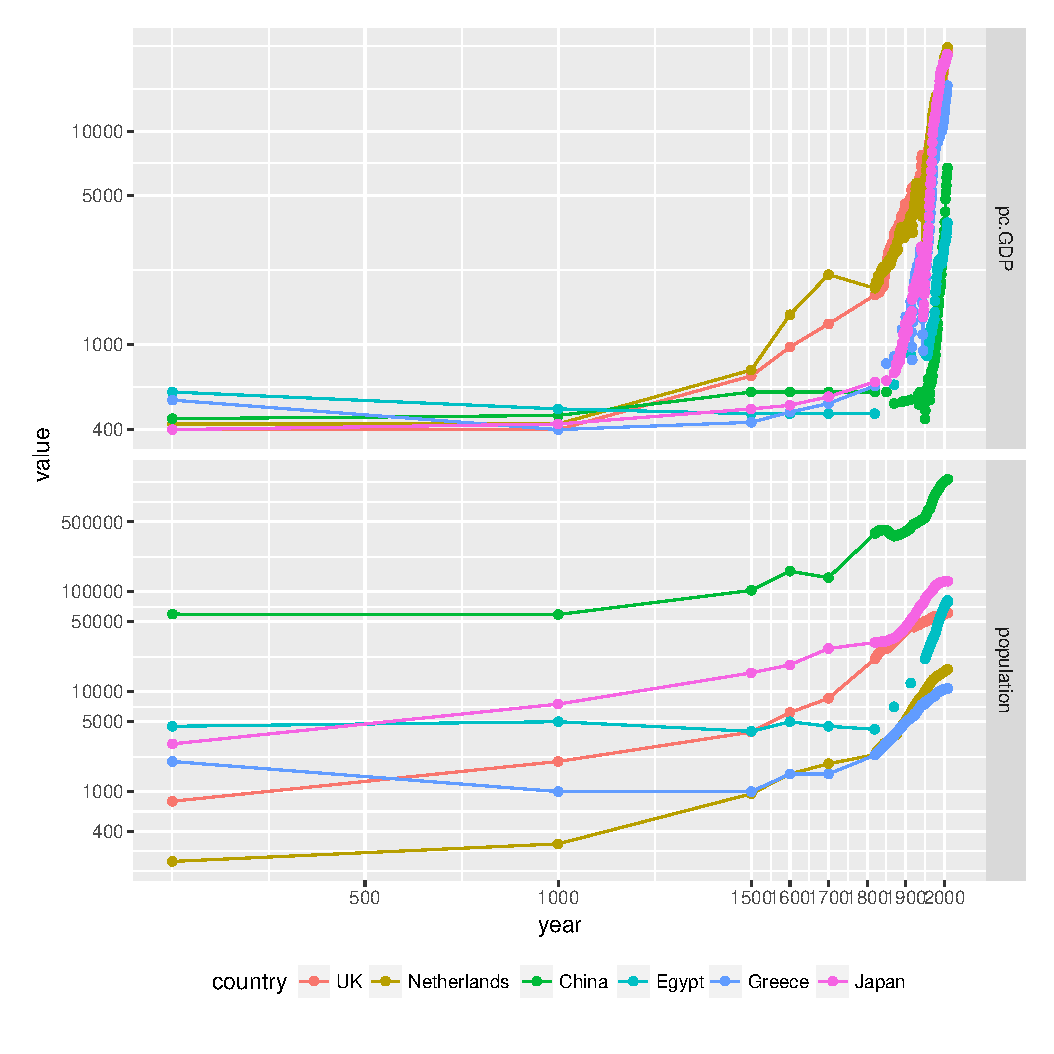
\includegraphics[clip, width = 12cm, height = 8cm]{1/world_income_pop_1-2009.eps}\\
Source: Angus Maddison.
\end{frame}
\begin{frame}{}
Per capita income since the beginning. (I made up \$200 in 40000BC.)\\
\hfil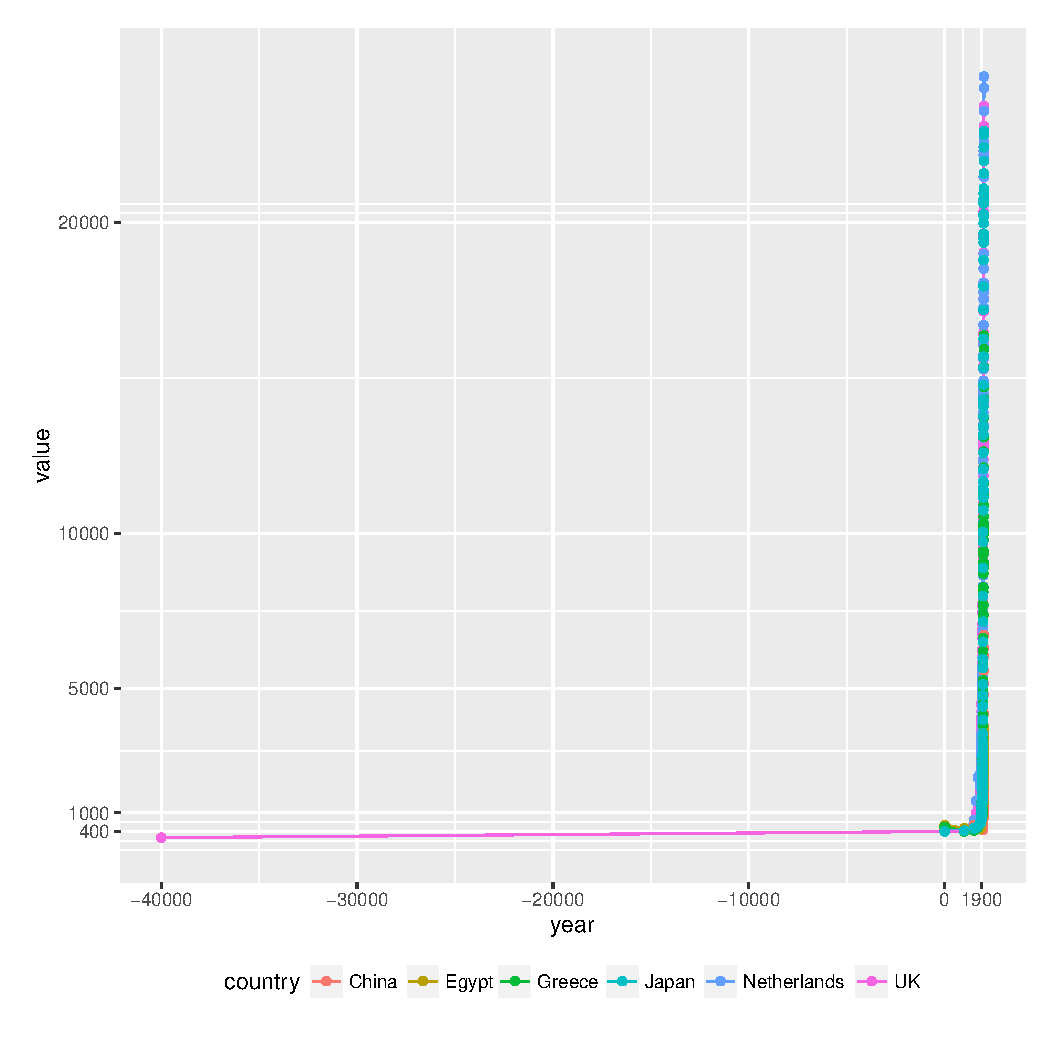
\includegraphics[clip, width = 12cm, height = 8cm]{1/world_income_pop_-40000-2009.eps}\\
Source: Angus Maddison.
\end{frame}

\begin{frame}{incomes across the globe}
次のページで1960年からの一人あたり所得が図に描かれています。どのようなパタンを予想しますか。\\
以下は2008年時点の一人あたり所得です。大きな格差です。1960年から差は縮まったでしょうか。\\
\hfil\setlength{\tabcolsep}{1pt}
\begin{tabular}{>{\scriptsize\hfil}p{.5cm}<{}>{\scriptsize\hfil}p{3cm}<{}>{\scriptsize\hfil}p{2cm}<{}>{\scriptsize\hfil}p{3cm}<{}>{\scriptsize\hfil}p{2cm}<{}}
\rowcolor{gray90}
\makebox[.5cm]{} & \makebox[3cm]{poorest} & \makebox[2cm]{poor USD} & \makebox[3cm]{richest} & \makebox[2cm]{rich USD}\\
1 & Zaire & 249 & Hong Kong & 31704\\
2 & Burundi & 479 & USA & 31178\\
3 & Niger & 514 & Norway & 28500\\
4 & Centr. Afr. Rep. & 536 & Singapore & 28107\\
5 & Comoro Islands & 549 & Ireland & 27898\\
6 & Togo & 606 & Australia & 25301\\
7 & Guinea Bissau & 617 & Canada & 25267\\
8 & Guinea & 628 & Switzerland & 25104\\
9 & Sierra Leone & 686 & Netherlands & 24695\\
10 & Haiti & 686 & Denmark & 24621
\end{tabular}

\end{frame}
\begin{frame}{incomes across the globe}
\begin{columns}[T]
\column{.8\textwidth}
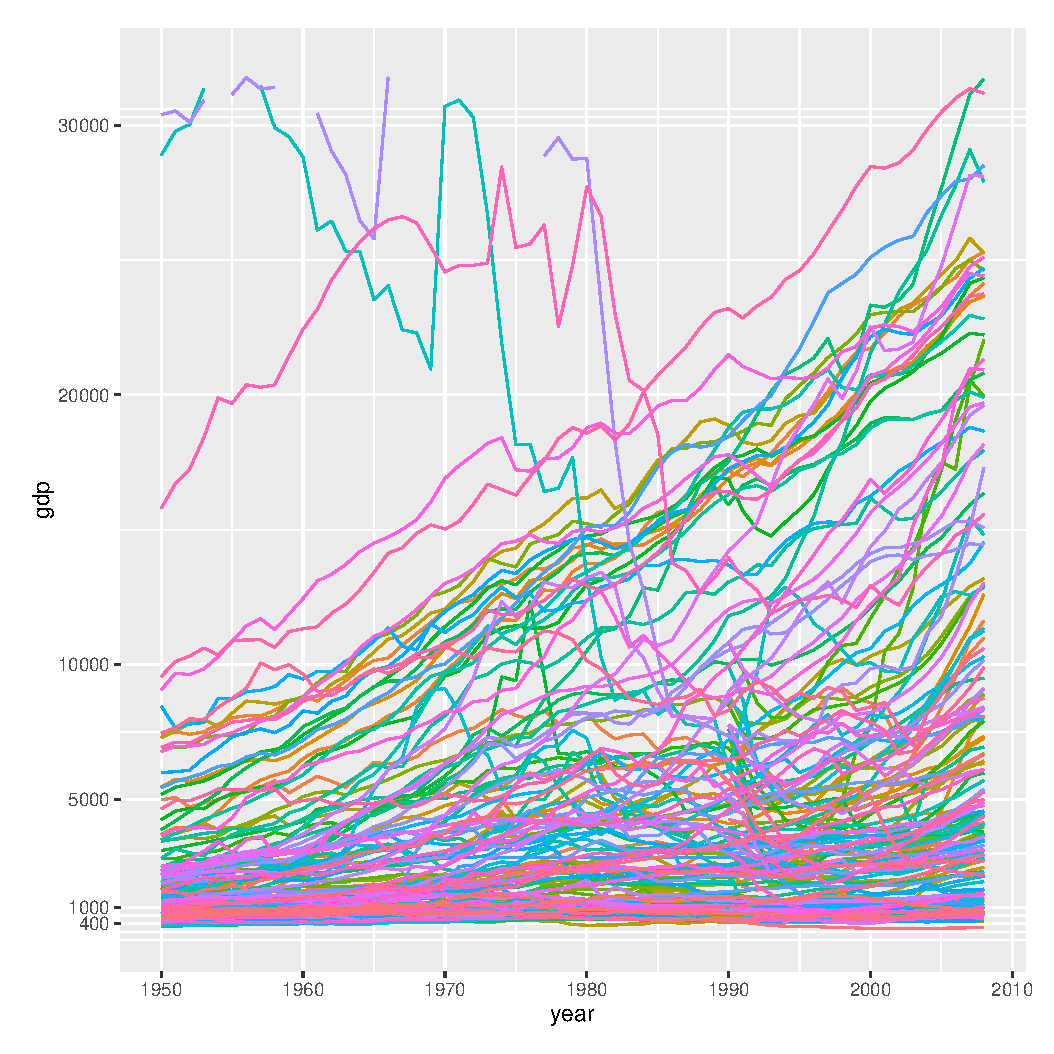
\includegraphics[clip, width = 12cm, height = 6cm]{1/world_income_1950-2008_natural.eps}\\
Source: Angus Maddison.
\end{columns}
\end{frame}
\begin{frame}{incomes across the globe}
\begin{columns}[T]
\column{.8\textwidth}
\hfil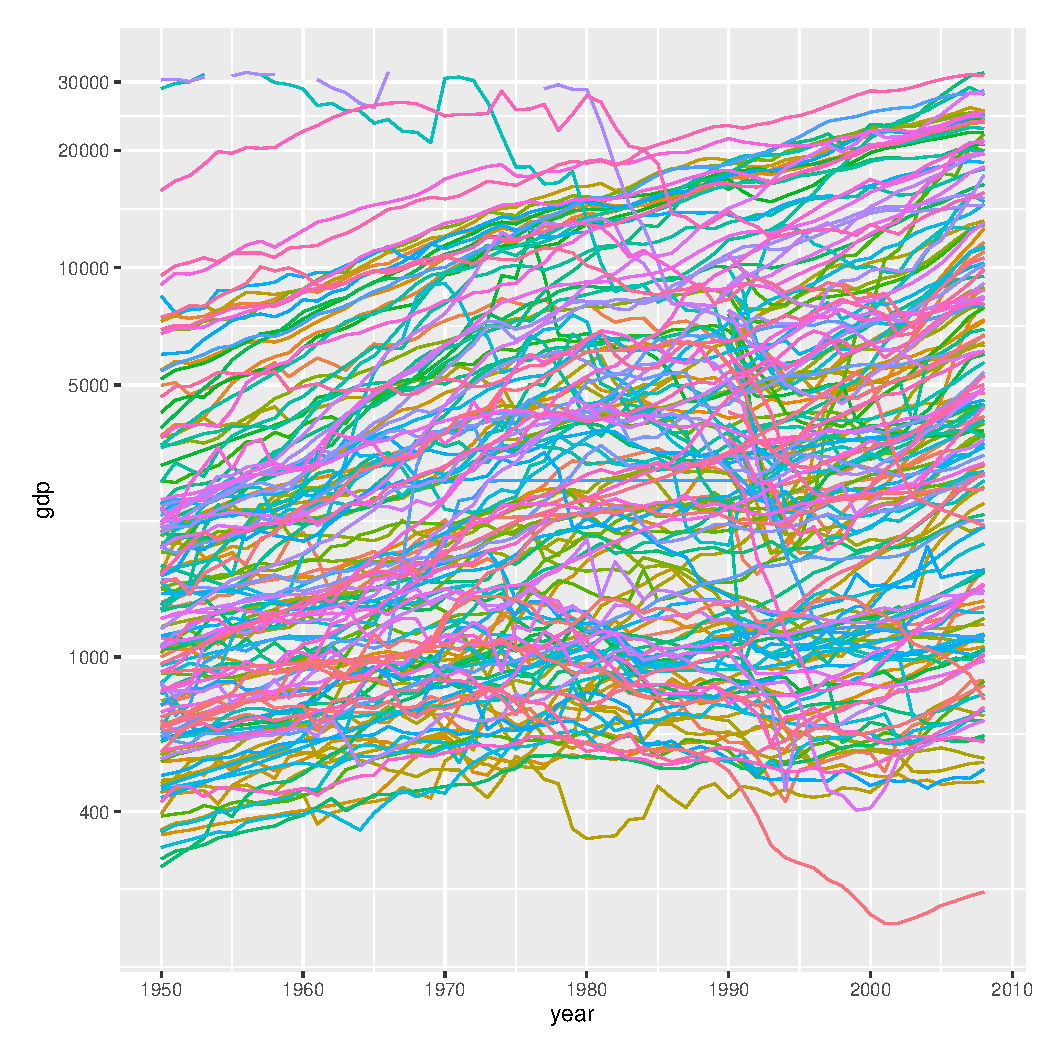
\includegraphics[clip, width = 12cm, height = 6cm]{1/world_income_1950-2008.eps}\\
Source: Angus Maddison.
\column{.2\textwidth}
Log scale does not give a clearer picture...
\end{columns}
\end{frame}








\begin{frame}{incomes across the globe, 1990-2020}
\begin{columns}[T]
\column{.8\textwidth}
\hfil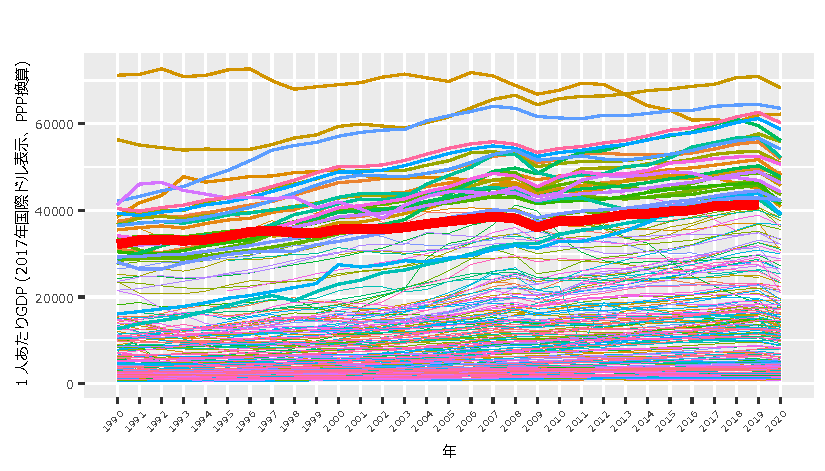
\includegraphics[clip, width = 12cm, height = 6.5cm]{c:/seiro/docs/external/seishin/lec_slides/2024/1/pcPPPGDP1990-2020.pdf}
\column{.2\textwidth}
\begin{itemize}
\vspace{1.0ex}\setlength{\itemsep}{1.0ex}\setlength{\baselineskip}{12pt}
\item	赤が日本
\item	2019年時点で日本よりも豊かな国は太線
\item	それ以外は細線
\item	(1990年に20000ドル以下で日本を追い抜いたのはマルタと韓国)
\end{itemize}
\end{columns}
Source: World Bank {\footnotesize \url{https://data.worldbank.org/indicator/NY.GDP.PCAP.PP.KD}}.\end{frame}
\begin{frame}{incomes across the globe, 1990-2020}
\begin{columns}[T]
\column{.8\textwidth}
\hfil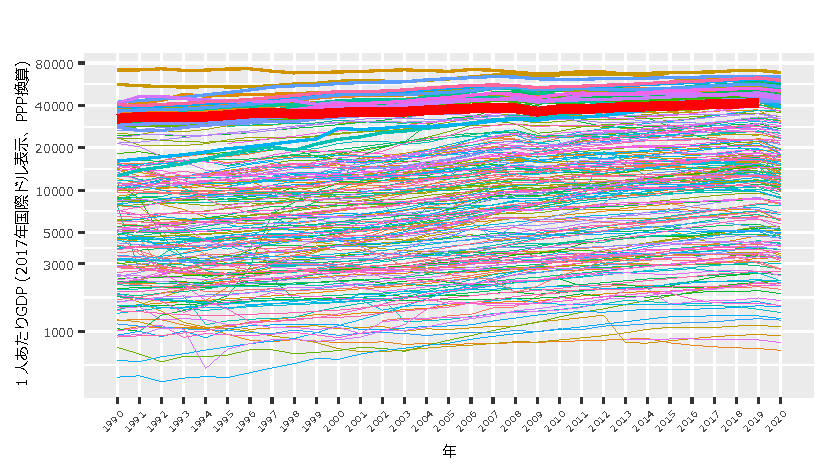
\includegraphics[clip, width = 12cm, height = 6.5cm]{c:/seiro/docs/external/seishin/lec_slides/2024/1/LogpcPPPGDP1990-2020.pdf}
\column{.2\textwidth}
\begin{itemize}
\vspace{1.0ex}\setlength{\itemsep}{1.0ex}\setlength{\baselineskip}{12pt}
\item	縦軸は対数目盛
\item	大きな値と小さな値を同時に表示するとき、対数目盛にすると小さい値がよりばらけて見える
\end{itemize}
\end{columns}
Source: World Bank {\footnotesize \url{https://data.worldbank.org/indicator/NY.GDP.PCAP.PP.KD}}.
\end{frame}

\begin{frame}[t, label=ConvergenceResults]{}
The message is clear.\\~\\
Poor countries are not catching up the rich countries.\\~\\
\pause
なお、1990年代以降は貧しい国も先進国にキャッチアップしつつあるという研究が最近出てきています\citep{KremerWillisYou2022}が、事実は認識されたものの、推計方法への注文が付いており\citep{AcemogluMolina2021}、ゆっくりキャッチアップしつつある理由、持続するかなど、解釈にはコンセンサスができていません。\hfill\hyperlink{NonConvergence}{\beamergotobutton{図}}\\~\\

\pause
国の平均値を比べるだけだと貧困が見落とされるという指摘もあります\citep{PandeEnevoldsen2021}。
\pause
中所得国になった国(インド、バングラデシュ、ナイジェリアなどの人口大国)にも多数の貧困層がいる、\pause
つまり、貧困問題を考えるために低所得国だけを対象にすると、多くの貧困層を見失います。\\~\\

低所得国と近かった中所得国が高所得国との差を縮めると各国間の所得不平等は減るが、中所得国がさらに高所得国に近づくと低所得国と中所得国の差が広がるため、いずれは各国間の所得不平等が増すという指摘もあります\citep{Kanbur2022}。
\end{frame}

\begin{frame}[label = WithinCountryInequality]{}
\begin{columns}[T]
\column{.35\textwidth}
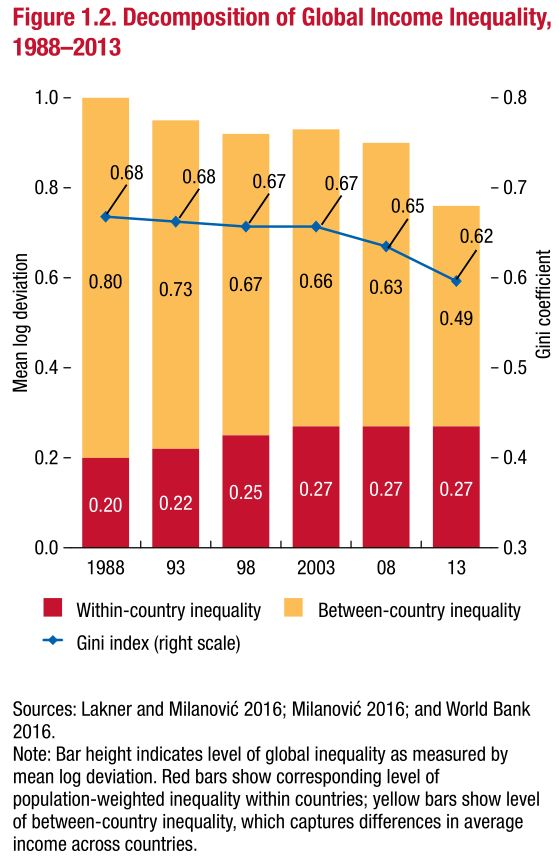
\includegraphics[width=\textwidth]{1/InequalityWithinBetweenCountries.jpg}\\
\column{.6\textwidth}
\pause
\footnotesize
Gini coefficientジニ係数: 分配の偏りを示す指標
\begin{description}
\vspace{.0ex}\setlength{\itemsep}{.0ex}\setlength{\baselineskip}{12pt}
\item[最小値は0]	全員が同じ所得を持つ状態
\item[最大値は1]	1人がすべての所得を持つ状態
\end{description}
\pause
\href{https://www.imf.org/-/media/Files/Publications/fiscal-monitor/2017/October/pdf/fm1702.ashx}{\citet{IMF2017Sep}}:\\
\begin{itemize}
\vspace{0.0ex}\setlength{\itemsep}{0.25ex}\setlength{\baselineskip}{12pt}
\item	全世界の所得分布のジニ係数: 0.68(1988)$\rightarrow$0.62(2013)
\pause
\item	国$c$個人$i$の(対数)所得$y_{ci}$と世界平均(対数)所得$\bar{y}$との差
=国間の差+国内の差
\[
y_{ci}-\bar{y}=\underbrace{\bar{y}_{c}-\bar{y}}_{\mbox{\scriptsize $c$国平均と世界平均の差}}+\underbrace{y_{ci}-\bar{y}_{c}}_{\mbox{\scriptsize 個人$i$と$c$国平均の差}}
\]
	\begin{itemize}\footnotesize
	\vspace{-3.0ex}\setlength{\itemsep}{1.0ex}\setlength{\baselineskip}{12pt}
\pause
	\item	国間格差: 0.80(1988)$\rightarrow$0.49(2013)
\pause
	\item	国内格差: 0.20(1988)$\rightarrow$0.27(2013)
	\end{itemize}
\end{itemize}
\pause
全体では格差は減ったが、国平均値の格差が減り、各国内の格差が増えた
\begin{dinglist}{43}
\vspace{.5ex}\setlength{\itemsep}{1.0ex}\setlength{\baselineskip}{12pt}
\pause
\item	低所得国で一部の人々が富裕になって低所得国の平均値は高まったが貧困層は残っている
\end{dinglist}
\end{columns}
\end{frame}

\begin{frame}{A simplified framework of development}
基本的な考え方: 貧困の罠poverty trap \pause (=複数均衡、複数のうち1つは歴史が決める低位均衡)
\begin{itemize}[<+->]
\vspace{1.0ex}\setlength{\itemsep}{1.0ex}\setlength{\baselineskip}{12pt}
\item	いかなる経済(コミュニティ)も豊かになり、成長してキャッチアップできる
\item	ただし、貧困の罠を脱出したとき\textit{のみ}
	\begin{dinglist}{43}
	\vspace{1.0ex}\setlength{\itemsep}{1.0ex}\setlength{\baselineskip}{12pt}
	\item	そうではなく、どの経済も順調に成長するなら政策は不要。放置でOK。
	\end{dinglist}
\item	貧困の罠の構成要素:
	\begin{enumerate}
	\vspace{1.0ex}\setlength{\itemsep}{1.0ex}\setlength{\baselineskip}{12pt}
	\item	1つ以上の均衡(通常は3つ)
	\item	低位均衡の動学的安定性dynamic stability(少しくらい所得が増えても減っても低位均衡に戻る性質、=悪循環a vicious cycle)
	\end{enumerate}
\end{itemize}
\end{frame}

\begin{frame}{A simplified framework of development}
\begin{columns}[T]
\column{.75\textwidth}
\onslide<1->{モデルの構成要素}
\begin{description}
\vspace{1.0ex}\setlength{\itemsep}{1.0ex}\setlength{\baselineskip}{12pt}
\item[資本$k_{t}$]	資本市場で供給$k^{S}_{t}$ = $k^{D}_{t}$需要 という状態の(物的、人的、社会共通、その他)資本. 
\end{description}
\begin{tikzpicture}[
  node distance = 2.5cm, align = flush center, font = \footnotesize, 
  on grid=false, inner sep=0pt, remember picture,
  every node/.style={minimum height = .5cm, minimum width = 1.75cm, text = blue}]
\onslide<2->{
  \node[fill = blue!30!white] (kt) at (0, 0) {$k_{t}$};
  \node[fill = blue!30!white, right of = kt] (prod) {生産=所得}; \node[fill = blue!30!white, right of = prod] (saving) {貯蓄}; \node[fill = blue!30!white, right of = saving] (kt1S) {供給$k^{S}_{t+1}$}; \node[fill = blue!30!white, right of = kt1S] (kt1) {$k_{t+1}$};
  \node[fill = blue!30!white, above of = kt1S, yshift = -1.5cm] (kt1D) {需要$k^{D}_{t+1}$};
%\node[fill = blue!30!white, right of = kt1D] (prodplan) {生産計画};
  \node[minimum width = 0em] (eq1) at ($ (kt1S) !.5! (kt1D) $) {\rotatebox{90}{$=$}};
  \node[minimum width = 0em] (eq2) at ($ (kt1S) !.5! (kt1) $) {$=$};
  \node[fill = white, text = black, minimum width = 0em] (tech) at ($ (kt) !.5! (prod) $) {};
  \node[fill = white, text = black, minimum width = 0em] (distrib) at ($ (prod) !.5! (saving) $) {};
  \node[fill = white, text = black, minimum width = 0em] (fin) at ($ (saving) !.5! (kt1S) $) {};
  \draw[->, >=stealth] (kt) -- (prod); 
  \draw[->, >=stealth] (prod) -- (saving); 
  \draw[->, >=stealth] (saving) -- (kt1S); 
}
\onslide<3->{
  \node[text = orange, above of = kt1, yshift = -1.5cm] (prodplan) {生産計画};
  \node[text = orange, left of = eq1] (capMeq) {資本市場均衡};
  \node[text = orange, below of = tech, yshift = 1cm] (techb) {生産技術};
  \node[text = orange, below of = distrib, yshift = .55cm] (distribb) {\mpage{1.75cm}{富の分布\\ 税制\\ マクロ経済}};
  \node[text = orange, below of = fin, yshift = 1cm] (finb) {金融制度};
  \draw[->, >=stealth, thick, blue] (techb) -- (tech); 
  \draw[->, >=stealth, thick, blue] (distribb) -- (distrib); 
  \draw[->, >=stealth, thick, blue] (finb) -- (fin); 
  \draw[->, >=stealth, thick, blue] (capMeq) -- (eq1); 
  \draw[<-, >=stealth, thick, blue] (kt1D) -- (prodplan); 
}
\onslide<4->{
  \draw[->, >=latex, thick, red] (kt) .. controls +(.1, -4.5) and +(-.1, -4.5) .. node[text = aqua, above] {$S$字線} (kt1); 
}
\end{tikzpicture}
\column{.25\textwidth}
\begin{itemize}
\vspace{1.0ex}\setlength{\itemsep}{1.0ex}\setlength{\baselineskip}{12pt}
\onslide<5->{
\item[S]	今期資本額$k_{t}$が与えられたときの来期資本額$k_{t+1}$を示す関係式。生産技術、富の分布、税制、マクロ経済の状態、金融制度、それらを支える法律や制度などが$k_{t+1}$に影響を及ぼす。
}
\end{itemize}

\end{columns}
%\item[(Walras' Law)]	General equilibrium \& capital market equilibrium \& labour market equilibrium $\Rightarrow$ Goods market equilibrium.
\end{frame}

\begin{frame}{A simplified framework of development}
\begin{columns}[T]
\column{.8\textwidth}
\onslide<1->{モデルの構成要素}
\onslide<2->{\begin{description}
\vspace{1.0ex}\setlength{\itemsep}{1.0ex}\setlength{\baselineskip}{12pt}
\item[資本]	資本市場で供給 = 需要 という状態の(物的、人的、社会共通、その他)資本. 
\end{description}}
\begin{itemize}
\vspace{1.0ex}\setlength{\itemsep}{1.0ex}\setlength{\baselineskip}{12pt}
\item<4->	今期資本$k_{t}$と生産・所得の関係 \onslide<5->{[資本需要; 経営、技術、$\cdots$]}
\item<6->	今期生産からどのくらい次期(t+1期)資本に増加されるか \onslide<7->{[資本増加分の供給; 貯蓄、富の分布、教育、$\cdots$]}
\item<8->	次期資本需要$k^{D}_{t+1}$と次期資本供給$k^{S}_{t+1}$ ($=$今期資本$k_{t}$ $+$ 今期貯蓄$s_{t}$)間の取引環境、今期資本$k_{t}$から次期資本$k_{t+1}$への時間を通じた変化: \onslide<9->{[市場と制度; 金融仲介、教育、規制、$\cdots$]}
\item<10->	人口で割って人口1人あたりの数にする \onslide<11->{[人口成長]}
\item<12->	資本市場均衡条件$k^{D}_{t+1}=k^{S}_{t+1}$を課す$\Rightarrow$ 方程式 (or 線)
\end{itemize}
\column{.2\textwidth}
\begin{itemize}
\vspace{1.0ex}\setlength{\itemsep}{1.0ex}\setlength{\baselineskip}{12pt}
\onslide<13->{\item[S]	S字形の直線で最低2つの尖端点があると最低3つの複数均衡
}
\onslide<14->{
\item	S字形は市場の不完全性などによって発生
}
\onslide<15->{
\item	S字形の曲線でも議論は同じ
}
\end{itemize}
\end{columns}
%\item[(Walras' Law)]	General equilibrium \& capital market equilibrium \& labour market equilibrium $\Rightarrow$ Goods market equilibrium.
\end{frame}

\begin{frame}{A simplified framework of development}
Next figure is based on \citet{GalorZeira1993}.
\end{frame}

\begin{frame}[label=DetailedPovTrapFig]{}
\setbeamercovered{invisible}
\input{1/PovertyTrap_DetailedDynamics.tkz}
\setbeamercovered{transparent}
\end{frame}


\begin{frame}[label=PovTrapFig]{A simplified framework of development}
\begin{columns}[T]
\column{.75\textwidth}
\input{1/poverty_trap.tkz}
\column{.25\textwidth}
\begin{itemize}
\vspace{1.0ex}\setlength{\itemsep}{1.0ex}\setlength{\baselineskip}{12pt}
\item	時間を通じた変化を考えること=動学dynamicsといいます
\item	動学では$t$時点と$t+1$時点の変化を考えます
\item	このモデルではキーとなる変数は一人あたり資本$k_{t}$なので、$k_{t}, k_{t+1}$平面で考えます
\end{itemize}
\hfill\hyperlink{WhyS<3>}{\beamergotobutton{S}}\hfill\hyperlink{changeequilibria<3>}{\beamergotobutton{Change equilibria}}
\\
\end{columns}
\end{frame}

\begin{frame}[label=WhyS]{A simplified framework of development}
なぜS字形?\pause 例(他の論拠もあります)\\~\\

\pause
発展段階・所得が低いときには生産性の伸びは低い。生産にさまざまな障害(市場の不完全性)があるため。資本蓄積の度合い(傾き)は緩やか。\hfill\hyperlink{PovTrapFig<5>}{\beamergotobutton{Figure}}
\begin{description}[市場に関わる制度]\footnotesize
\vspace{1.0ex}\setlength{\itemsep}{1.0ex}\setlength{\baselineskip}{12pt}
\pause
\item[資本市場] 借り手と貸し手が出会う機会が乏しい、資金回収リスクがあるので資金を提供しにくい
\pause
\item[保険市場] 灌漑施設と降雨保険がないと、乾燥に強い低収益作物(アワ、ヒエ)
\pause
\item[貸出市場] 子どもの教育投資は家計の豊かさに依存するので、低所得家計は投資しにくい
\pause
\item[市場に関わる制度] 司法、行政、インフラなどが不十分で投資収益が下がる\\~\\
\end{description}
\pause
発展段階・所得が中段階になると生産性の伸びが高まる。市場が整備され、豊かな国からの技術移転も利用できるため。資本蓄積の度合い(傾き)は急。\\~\\

\pause
発展段階・所得が高くなると、生産性の伸びは低くなる。技術移転に頼らず自前で技術開発しないといけなくなるから。資本蓄積の度合い(傾き)は緩やか。
\hfill\hyperlink{PovTrapFig<5>}{\beamergotobutton{Figure}}
\end{frame}

\begin{frame}[label = changeequilibria]{A simplified framework of development}
資本市場均衡線がS字直線で、極端に高い位置や低い位置にない限り、45度線と3つ交点を持つ
\begin{dinglist}{43}
\vspace{1.0ex}\setlength{\itemsep}{1.0ex}\setlength{\baselineskip}{12pt}
\pause
\item	厳密には、S字直線の緩やかな傾きが45度未満、急な傾きが45度以上で、Sの下部分が45度線よりも高い位置で始まり、急な傾きになる前に1つ交点を持てば、合計で3つ交点を持つ\\~\\
\end{dinglist}
\pause
経済が動学的に安定な低位均衡にいると、高位均衡には自然に移らない。
\begin{itemize}[<+->]
\vspace{1.0ex}\setlength{\itemsep}{3.0ex}\setlength{\baselineskip}{12pt}
\item	$H$に行くためには以下が必要:
	\begin{enumerate}[<+->]
	\vspace{1.0ex}\setlength{\itemsep}{1.0ex}\setlength{\baselineskip}{12pt}
	\item	 $S$線を引き上げて高位均衡への収束経路に乗せる制度変化。
\hfill\hyperlink{shiftedS<1>}{\beamergotobutton{Figure}}\\
	\item	経済を一気に右側に移して高位均衡への収束経路に乗せるビッグ・プッシュ。 大量の資本$k$を投下 (``マーシャル・プラン''). 
\hfill\hyperlink{PovTrapFig<22>}{\beamergotobutton{Figure}}
	\end{enumerate}
\item	どの制度を変化させるか? どの資本を増やすか? どうやって?
\end{itemize}
\end{frame}


\begin{frame}{How to learn}
J-PAL to the rescue!
\begin{itemize}[<+->]
\vspace{1.0ex}\setlength{\itemsep}{1.0ex}\setlength{\baselineskip}{12pt}
\item	Abdul Ratif Jameel Poverty Action Lab at MIT.
\item	\sout{Homepage: ``729 ongoing and completed randomized evaluations in 67 countries''.}
\item	``1094 randomized evaluations...in 91 countries,'' ``from clean water to microfinance to crime prevention.'' 
\item	大変な数
\item	ランダム化比較試験RCTは政策の効果を歪み無く示すことができる
	\begin{itemize}
	\vspace{1.0ex}\setlength{\itemsep}{1.0ex}\setlength{\baselineskip}{12pt}
	\item	なぜ歪まないか? 理由はコースの後半で学びます。
	\end{itemize}
\item	RCTはパイロット研究pilot studyです。パイロット研究はロジスティクスや費用対効果などを示すことができます。
\end{itemize}
\end{frame}

\begin{frame}{}
Examples: A summary of their RCTs on \href{https://www.povertyactionlab.org/policy-lessons/education/increasing-test-score-performance}{learning (web page in 2020)}.
\begin{itemize}[<+->]
\vspace{1.0ex}\setlength{\itemsep}{1.0ex}\setlength{\baselineskip}{12pt}
\item	When access to education is extremely limited, getting children into school can lead to large learning gains (Afghanistan).
\item	Motivating students to go to school and learn can be very cost-effective, by scholarship (Kenya), by conditional cash transfer (Malawi).
\item	There is little evidence that simply increasing the number of teachers or teaching resources improves learning (India, Kenya, Kenya, Kenya). 
\item	Teaching children according to their actual learning levels is the most consistently effective at improving learning, and is also very cost-effective (Kenya, Kenya, India, India).
\end{itemize}
\end{frame}

\begin{frame}{}
Examples: Learning (continued).
\begin{itemize}
\vspace{1.0ex}\setlength{\itemsep}{1.0ex}\setlength{\baselineskip}{12pt}
\item	Incentives for teachers can lead to significant learning gains if they are objectively administered and structured in such a way as to discourage ``teaching to the test'' (India, Kenya, India).
\item	Adding an extra teacher on a short-term contract can produce significant learning gains at a relatively low cost (Kenya).
\item	Grants provided to communities as part of empowerment programs can lead to better learning (Gambia, Indonesia).
\end{itemize}
%Finally! We have a country other than India and Kenya.
\end{frame}

\begin{frame}{}
ここで変なことは何でしょう? OK, what is wrong with this picture?
\setbeamercovered{invisible}
\pause
\begin{itemize}
\vspace{1.0ex}\setlength{\itemsep}{1.0ex}\setlength{\baselineskip}{12pt}
\item	途上国はインドとケニアだけではありません
\item	(Not shown) J-PALは一緒に仕事する組織が当然限られます。India = Maharashtra, Telangana, Rajasthan; Kenya = 西部の州.
\item	``India'' $\neq$ India, ``India'' $=$ 少数の州. ``Kenya''も同じ
\end{itemize}
\pause
\begin{dinglist}{43}
\vspace{1.0ex}\setlength{\itemsep}{1.0ex}\setlength{\baselineskip}{12pt}
\item	政策効果の因果推計causal inference (教訓the lesson learned)が他の地域に当てはまらないとき、推計は\textcolor{pink}{外的妥当性external validity}を欠く、といいます。リストした研究内容は外的妥当性が限られています。 
\item	推計が因果関係を捉えている(識別するidentify)とき、推計には\textcolor{pink}{内的妥当性internal validity}がある、といいます。
\end{dinglist}
\pause
\begin{itemize}
\vspace{1.0ex}\setlength{\itemsep}{1.0ex}\setlength{\baselineskip}{12pt}
\item	これは厳しすぎる批判かも。J-PALは重要な知見のある研究をたくさん実施。
\item	しかし、リスト内容からは、小規模RCTを使った方法に限界があることが分かります。
\item	 \alt<5->{2019年にJ-PALのBanerjee, Duflo, Kremerがノーベル経済学賞を受賞。}{\sout{彼らはノーベル平和賞\textit{と}ノーベル経済学賞を受賞すべきです。}} 
\end{itemize}
\setbeamercovered{transparent}
\end{frame}

\begin{frame}{}
彼らの研究の集大成: \textit{Poor Economics} written by \citet{BanerjeeDuflo2011book}.
\begin{dinglist}{43}
\pause
\vspace{1.0ex}\setlength{\itemsep}{1.0ex}\setlength{\baselineskip}{12pt}
\item	素晴らしい本。読みやすい。開発経済学に興味のある誰もが読むべき。
\end{dinglist}

\vspace{1ex}
\pause
\citet{Ravallion2012,Rosenzweig2012}は批判:
\begin{itemize}
\vspace{1.0ex}\setlength{\itemsep}{1.0ex}\setlength{\baselineskip}{12pt}
\item	小規模なエビデンスを積み上げるとビッグ・プッシュになるのか?
\pause
\begin{dinglist}{43}
\vspace{1.0ex}\setlength{\itemsep}{1.0ex}\setlength{\baselineskip}{12pt}
\item	的を射ている。他の研究方法と組み合わせれば良いのでは?
\pause
\item	行政データなどの大規模データを使った観察研究でも知見はある。
\end{dinglist}
\end{itemize}

\vspace{1ex}
\pause
\citet{HeckmanSmith1995, Heckman2010bridgegaps}はRCTの利用と誘導型推計を疑問視:
\begin{itemize}[<+->]
\vspace{1.0ex}\setlength{\itemsep}{1.0ex}\setlength{\baselineskip}{12pt}
\item	全ての政策を実験・ランダム化できるのか? できない。
\item	ランダム化=政策実施か? 二重盲検(double blind) RCTでないと、ランダム化バイアスrandomisation biasは必ずある。
\item	なぜ効果があった・無かったのか? メカニズムを示す理論はあるのか?
	\begin{dinglist}{43}
	\vspace{1.0ex}\setlength{\itemsep}{1.0ex}\setlength{\baselineskip}{12pt}
	\item	ただし、誘導型推計でも理論を検定することは可能
	\end{dinglist}
\end{itemize}
\end{frame}

\begin{frame}{}
彼らによれば\citep{BanerjeeDuflo2011book}、彼らの研究の前は貧困には2つのアプローチがありました。
\pause
\begin{description}[<+->]
\vspace{1.0ex}\setlength{\itemsep}{1.0ex}\setlength{\baselineskip}{12pt}
\item[Save them.] 助けが必要 ... a Big Push \citep{Sachs2006}。Milleneum Village Project.
\item[Can't save them.] 放っておこう。自分たちで豊かにならないといけない\citep{Easterly2006}。
\end{description}

\vspace{1ex}
\pause
\citet{BanerjeeDuflo2011book}は中間を示したと主張します。\textit{Poor Economics}以前の時代を単純化しすぎていないか、ちょっと疑問が残ります。
\end{frame}

\begin{frame}{}
\href{http://millenniumvillages.org/}{Milleneum Villages}はどうなったでしょうか? \href{http://www.odi.org/projects/765-millennium-villages-project-review}{ODI's review page}の引用.
\pause
\begin{quotation}
The project is led by Professor Jeffrey Sachs of the Earth Institute, Columbia University. The five year project was launched in 2006 and targets 80 Millennium Villages across ten African countries. It provides low-cost interventions in agriculture and nutrition, health, water and sanitation, education, infrastructure and the environment to the villages at a cost of \$120 per person per year.

\pause
(In summary) The MVP has achieved results and has demonstrated the impact of greater investment in evidence-based, low-cost interventions at village level on progress towards the MDGs. 
\end{quotation}

\pause
レビューはポジティブな内容です。その回答Sachs et al. (2008)は感謝していました。
\end{frame}

\begin{frame}{A simplified framework of development}
\begin{itemize}[<+->]
\vspace{-1.0ex}\setlength{\itemsep}{1.0ex}\setlength{\baselineskip}{12pt}
\item	サックスはMV Project \href{https://www.project-syndicate.org/commentary/jeffrey-d-sachs-defends-the-track-record-of-the-millennium-villages-project}{``is flourishing''}といいます。
\item	Bill Gatesはサックスを賞賛しているものの(\href{https://www.project-syndicate.org/commentary/bill-gates-explains-why-the-millennium-villages-project--though-a-failure--was-worth-the-risk}{``Sachs is the Bono of economics''})、MVPの成果に批判的です。\hfill\href{https://www.rte.ie/archives/exhibitions/937-u2/291767-bono-remembers-the-early-years/}{\footnotesize Bono1}, \href{https://upload.wikimedia.org/wikipedia/commons/6/60/Bush_and_Bono.jpg}{\footnotesize Bono2}
\item	しかし...成果についてなぜ意見が割れるのでしょうか。だって、成果に関するデータをチェックすれば1は1、2は2なので意見を異にする点はないのでは?
\item	答え: MV Projectの評価デザインに本質的な欠点がある(see \href{http://www.economist.com/blogs/feastandfamine/2012/05/jeffrey-sachs-and-millennium-villages}{The Economist article})ので、見方が割れます。
	\begin{dinglist}{43}
	\vspace{1.0ex}\setlength{\itemsep}{1.0ex}\setlength{\baselineskip}{12pt}
	\item	サックスは天才なので、彼がなぜこんなデザインにしたのか不思議です。
	\item	もしかすると、自由にデザインを選べなかったのかも ... コースの後半で扱います。
	\end{dinglist}
\item	この講義では、欠点が何か、修正する方法を学びます。
\end{itemize}
\end{frame}

\begin{frame}{key words}
\begin{description}[<+->]
\vspace{1.0ex}\setlength{\itemsep}{1.0ex}\setlength{\baselineskip}{12pt}
\item[Poverty trap] A vicious cycle that keeps the economy in poverty.
\item[Big Push] A set of policies that moves the economy to a convergent path to ``high'' equilibria.
\item[Milleneum Development Villages] An attempt to mimic a Big Push that intervenes the African villages in every aspect of life.
\item[J-PAL] A research centre focusing on randomised controlled trials (RCTs) to produce practical policy lessons.
\item[internal validity] An unbiased causal inference.
\item[external validity] An unbiased causal inference with applicability beyond studied subjects.
\end{description}
\end{frame}

\begin{frame}[allowframebreaks]{References}
\scriptsize
\setlength{\baselineskip}{8pt}
\bibliographystyle{aer}
\bibliography{c:/seiro/settings/TeX/seiro.bib}
\end{frame}


\begin{frame}[label = shiftedS]{A simplified framework of development}
\input{1/poverty_trap2.tkz}\\
\hfill\hyperlink{changeequilibria<4>}{\beamergotobutton{go back}}
\end{frame}

\begin{frame}[label = PovTrapEmpirics]{}
\begin{columns}[T]
\column{.65\textwidth}
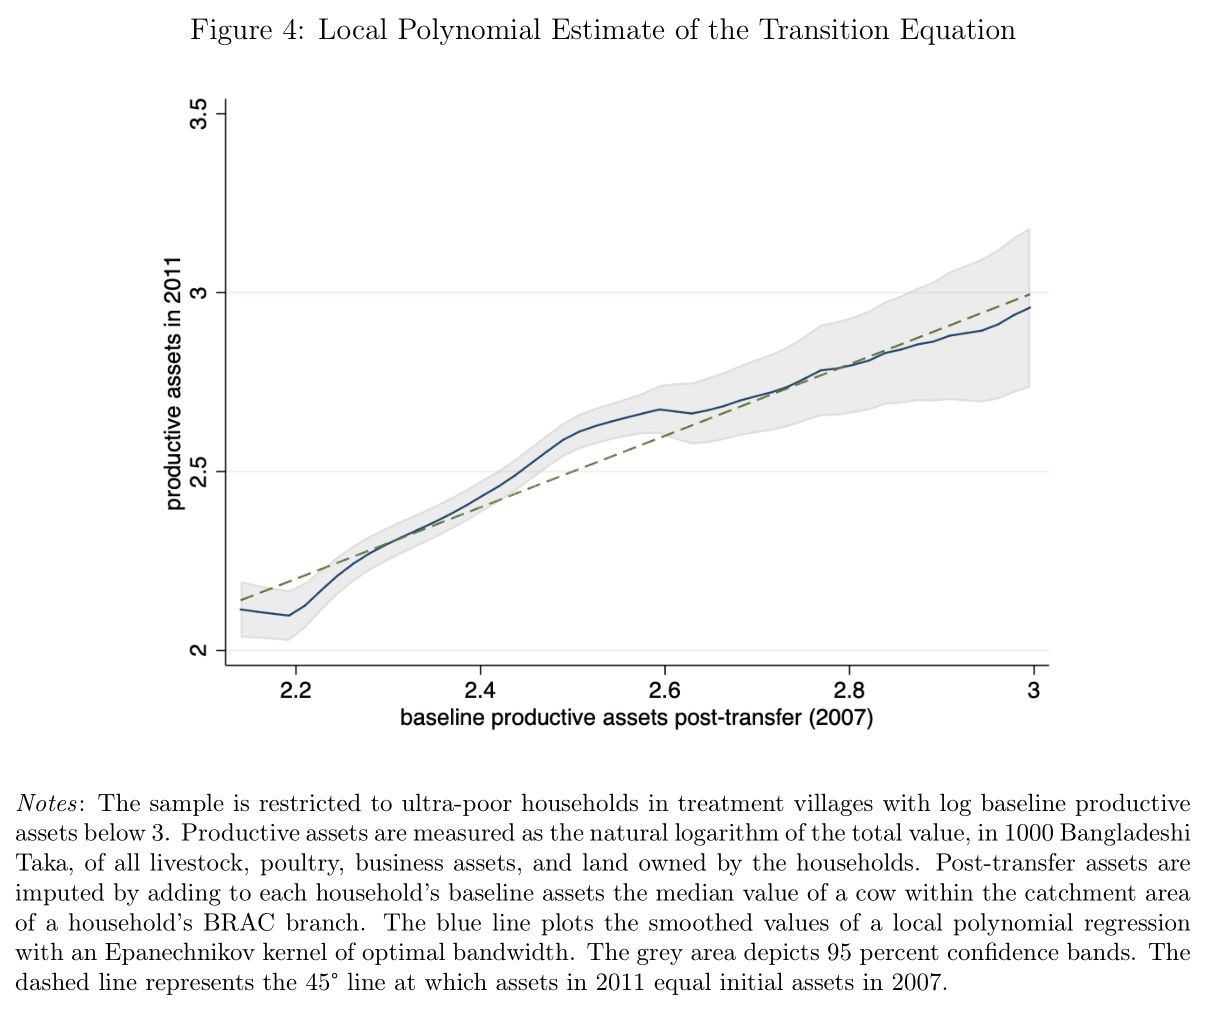
\includegraphics[width=.65\paperwidth]{c:/seiro/docs/external/seishin/lec_slides/2024/1/Balboni_PovTrapFig.jpg}
\column{.3\textwidth}
\begin{itemize}\scriptsize
\vspace{1.0ex}\setlength{\itemsep}{1.0ex}\setlength{\baselineskip}{12pt}
\item	点線が45度線、曲線が家計調査で情報収集した家計資産を2007年($=k_{t}$)と2011年($=k_{t+1}$)で描いたものです\citep[][Figure 4]{Balboni2020}。緩やかなS字曲線が分かります。貧困の罠をデータで実証した研究は、おそらくこれが初めてです。
\item	伊藤も共著者たちと一緒にバングラデシュ北部で似た研究をして、最貧困層へのビッグプッシュ的介入(マイクロファイナンスの多額貸付)が家計資産蓄積を加速させることを発見しました。
\end{itemize}
\end{columns}

\hfill\hyperlink{changeequilibria<4>}{\beamergotobutton{go back}}
\end{frame}

\begin{frame}[label=PeterSingerEnglish]{}
Peter Singer, an ethicist, a philospher. \\~\\

\href{https://www.thelifeyoucansave.org.au/child-in-the-pond/}{\textit{Child in the pond} question:}\\

\begin{quotation}
You are walking in an isolated park, passing by a pond, where you see a child drowning. There is no one around, and you do not have a phone to call for a help. You are good at swimming and can save the child by jumping into the water. But you have expensive shoes on. Jumping into the water will ruin them, a loss of USD 200. If you do not help the child, the child will die.\\~\\
\end{quotation}


Would you jump into the pond to save the child?\\~\\
\hfill\hyperlink{PeterSinger<2>}{\beamergotobutton{go back}}
\end{frame}

\begin{frame}{}
Almost everybody (probably everybody in developed countries) will say, yes. \\~\\

Singer challenges: Then, why would you not give USD 200 to help a child on the other side of globe?\\~\\

Singer argues that we, citizens of a rich nation, are morally obligated to give a fraction of income to the citizens of poor nations. \\~\\

We want to be empathetic, but we are so incapable of being so, of thinking about the poverty in poor countries. We may have to force ourselves to think about it.
\end{frame}

\begin{frame}[label = NonConvergence]{}
\begin{columns}[T]
\column{.8\textwidth}
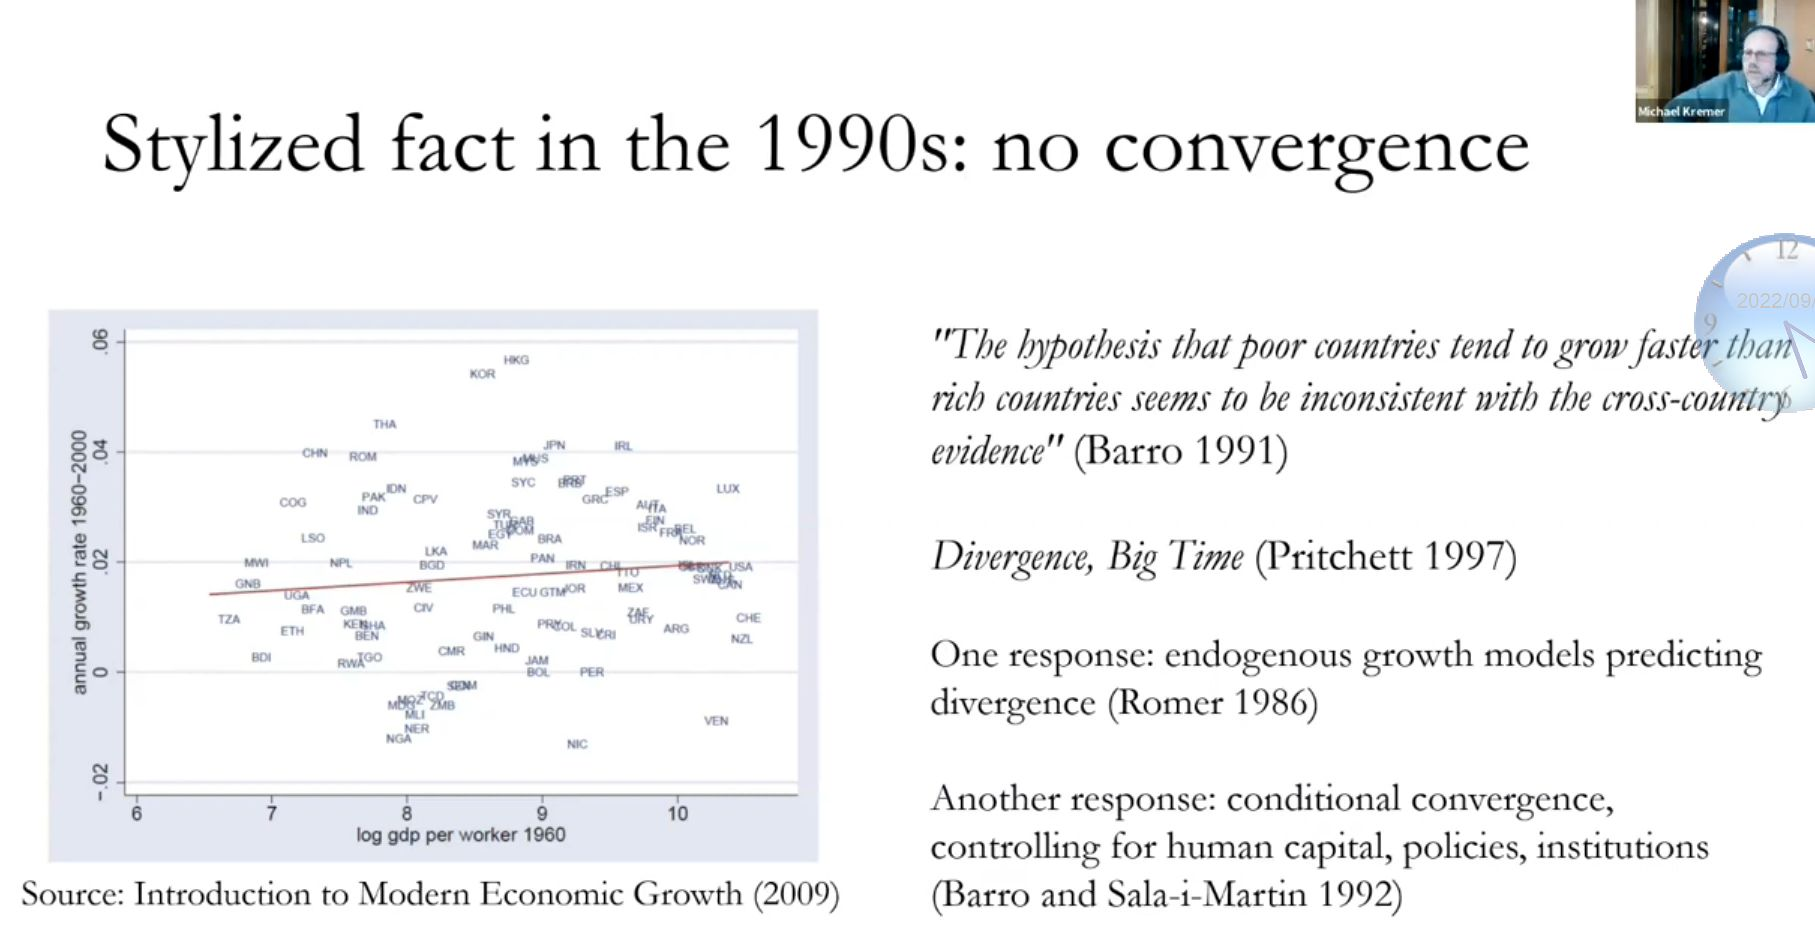
\includegraphics[width=12cm]{1/NonConvergence.jpg}\\
\column{.2\textwidth}
経済成長理論の入門教科書の図\\~\\
convergence=収斂、キャッチアップ\\~\\
\pause
キャッチアップするには所得の低い国ほど成長率が高い必要あり\\~\\
\end{columns}
%\hfill\hyperlink{ConvergenceResults<2>}{\beamergotobutton{go back}}
\pause
横軸1960年の1人当たり対数所得、縦軸1960-2000年成長率とすると、右下がりの関係が必要\\~\\
\pause
僅かに右上がり=キャッチアップなし
\end{frame}

\begin{frame}[label = ConvergenceIn2000]{}
\begin{columns}[T]
\column{.8\textwidth}
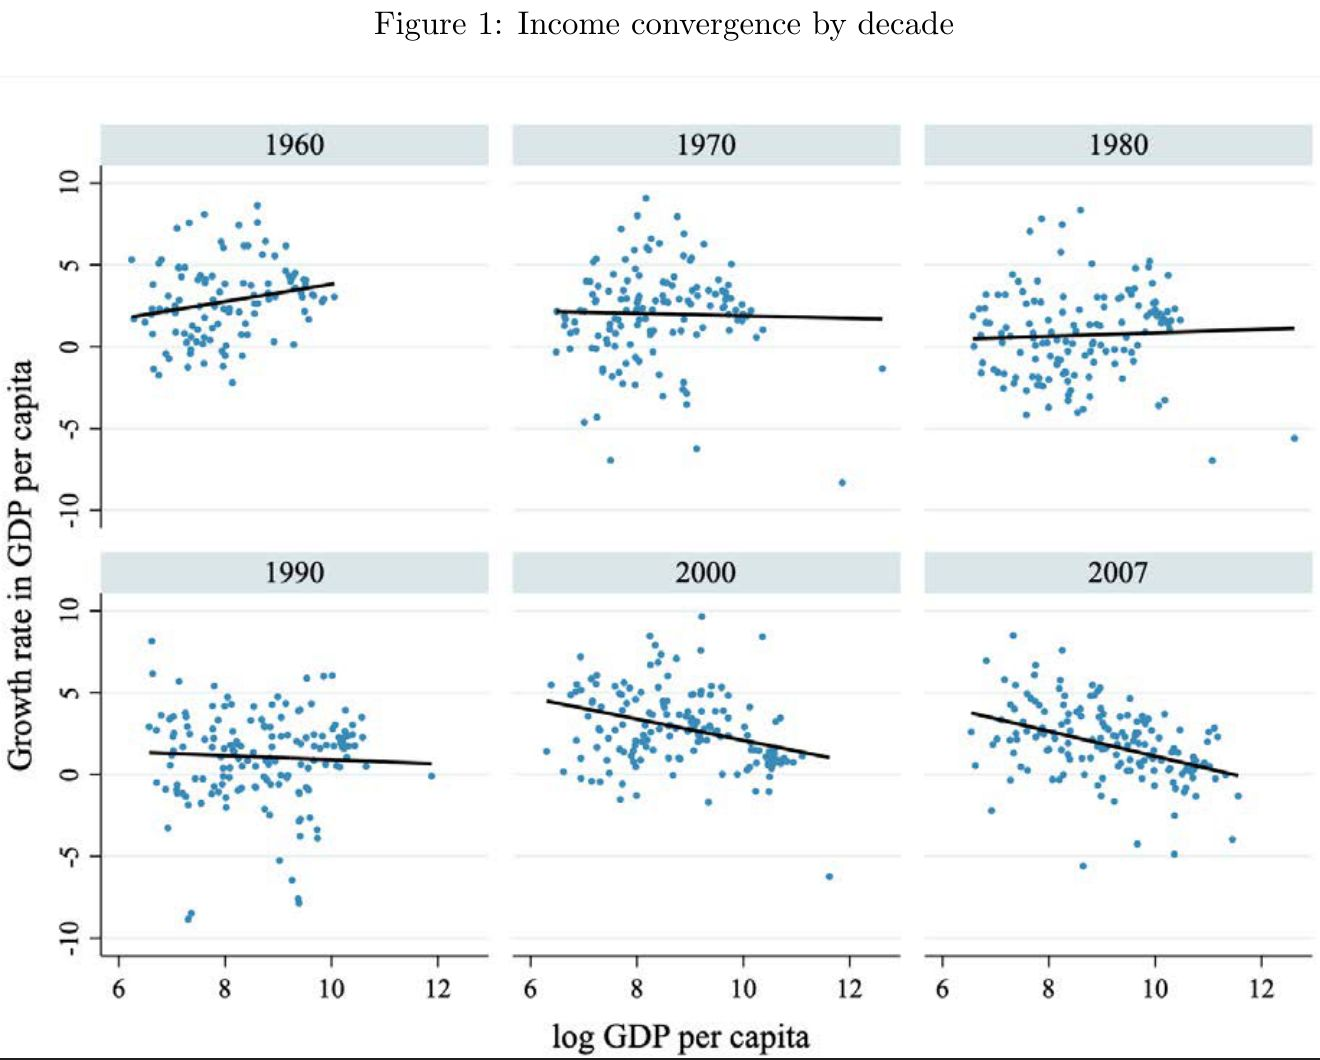
\includegraphics[width=12cm]{1/ConvergenceIn2000s.jpg}\\
\column{.2\textwidth}
\citet{KremerWillisYou2022}\\~\\
2007: 2007-2017\\
\hfill\hyperlink{ConvergenceResults<2>}{\beamergotobutton{go back}}
\end{columns}
\end{frame}

\end{document}

